%====================================================================================================
%  DMS 2.0 -- Reference manual and user guide
%  Compile: pdflatex dms_manual.tex (twice, for the table of contents and cross references)
%====================================================================================================
\documentclass[11pt,a4paper]{article}

\usepackage[utf8]{inputenc}
\IfFileExists{lmodern.sty}{\usepackage[T1]{fontenc}\usepackage{lmodern}}{}
\usepackage[margin=2.4cm]{geometry}
\usepackage{amsmath,amssymb}
\usepackage{microtype}
\usepackage{booktabs,longtable,tabularx,array}
\usepackage{enumitem}
\usepackage{xcolor}
\usepackage{listings}
\usepackage{tikz}
\usetikzlibrary{arrows.meta,positioning,calc}
\usepackage{caption}
\usepackage{placeins}
\usepackage{fancyhdr}
\usepackage[hidelinks]{hyperref}

\definecolor{codebg}{RGB}{246,246,243}
\definecolor{codeframe}{RGB}{205,205,198}
\definecolor{accent}{RGB}{30,80,140}

\lstdefinestyle{base}{
  basicstyle=\ttfamily\small, backgroundcolor=\color{codebg}, frame=single,
  rulecolor=\color{codeframe}, framesep=4pt, xleftmargin=6pt, xrightmargin=6pt,
  columns=fullflexible, keepspaces=true, showstringspaces=false, breaklines=true,
  aboveskip=8pt, belowskip=8pt, commentstyle=\color{gray}\itshape, upquote=true}
\lstdefinestyle{nml}{style=base, basicstyle=\ttfamily\footnotesize, morecomment=[l]{!}, morestring=[b]'}
\lstdefinestyle{sh}{style=base, morecomment=[l]{\#}}
\lstdefinestyle{py}{style=base, language=Python, keywordstyle=\color{accent}\bfseries}
\lstset{style=base}

\newcommand{\dms}{\textsc{dms}}
\newcommand{\code}[1]{\texttt{#1}}
\newcommand{\um}{\,$\mu$m}
\newcommand{\dd}{\mathrm{d}}
\newcommand{\Msun}{M_\odot}

\setlist{itemsep=2pt, topsep=4pt}
\setlength{\parskip}{3pt}
\renewcommand{\arraystretch}{1.15}
\newcolumntype{R}[1]{>{\raggedright\arraybackslash}p{#1}}
\setlength{\emergencystretch}{3em}

\pagestyle{fancy}
\fancyhf{}
\fancyhead[L]{\small DMS 2.0 manual}
\fancyhead[R]{\small\nouppercase{\leftmark}}
\fancyfoot[C]{\small\thepage}
\renewcommand{\headrulewidth}{0.4pt}

%----------------------------------------------------------------------------------------------------
% Cover. The eight images are in cover/images/ (made with cover/cover_models.py and
% cover/cover_images.py). Positions are fractions of the paper width (x) and height (y), measured
% from the lower left corner; the text is set in Helvetica (helvet, part of every TeX installation).
\definecolor{covertext}{HTML}{D8DDE6}
\definecolor{coversub}{HTML}{B9C2D0}
\definecolor{covergrey}{HTML}{8B93A3}
\definecolor{covernote}{HTML}{6D7585}
\newcommand{\coverfont}{\fontfamily{phv}\selectfont}
\newcommand{\coverat}[2]{($(current page.south west)+({(#1)*\paperwidth},{(#2)*\paperheight})$)}
\newlength{\coverpanelwidth}
% \coverpanel{x}{y}{image}{caption}{second line}: image with its lower left corner at (x, y)
\newcommand{\coverpanel}[5]{%
  \node[anchor=south west, inner sep=0pt] at \coverat{#1}{#2}
    {\includegraphics[width=\coverpanelwidth]{cover/images/#3}};
  \node[anchor=north west, inner sep=0pt, text=covertext, font=\coverfont\fontsize{7.5}{9}\selectfont]
    at \coverat{#1+0.005}{#2-0.008} {#4};
  \node[anchor=north west, inner sep=0pt, text=covergrey, font=\coverfont\fontsize{6.2}{8}\selectfont]
    at \coverat{#1+0.005}{#2-0.0205} {#5};}

\hypersetup{pdftitle={DMS 2.0: Reference manual and user guide}, pdfauthor={Minjae G. Kim}}

\begin{document}

%----------------------------------------------------------------------------------------------------
% Cover
\pagenumbering{Alph}
\begin{titlepage}
\setlength{\coverpanelwidth}{0.1965\paperwidth}
\begin{tikzpicture}[remember picture, overlay]
  \fill[black] (current page.south west) rectangle (current page.north east);
  % title
  \node[anchor=north west, inner sep=0pt, text=white, font=\coverfont\bfseries\fontsize{60}{66}\selectfont]
    at \coverat{0.08}{0.93} {DMS 2.0};
  \node[anchor=north west, inner sep=0pt, text=white, font=\coverfont\fontsize{19}{23}\selectfont]
    at \coverat{0.08}{0.848} {Debris disks around Main-sequence Stars};
  \node[anchor=north west, inner sep=0pt, text=coversub, font=\coverfont\fontsize{13}{16}\selectfont]
    at \coverat{0.08}{0.812} {Reference manual and user guide};
  % images: four columns (x = 0.08 + i (0.1965 + 0.018)), two rows (y = 0.50 and 0.27)
  \coverpanel{0.08}{0.50}{ring_sca}{Scattered light, 1.6\,\textmu m}{narrow ring, \textit{i}\,=\,76\textdegree}
  \coverpanel{0.2945}{0.50}{ring_qphi}{Polarised light \textit{Q}$_\phi$, 1.6\,\textmu m}{same ring}
  \coverpanel{0.509}{0.50}{edge_on}{Edge-on disk, 1.6\,\textmu m}{\textit{i}\,=\,87\textdegree}
  \coverpanel{0.7235}{0.50}{two_belts}{Two belts, 24 / 70 / 870\,\textmu m}{warm inner, cold outer belt}
  \coverpanel{0.08}{0.27}{peri}{Pericentre glow, 24\,\textmu m}{\textit{e}\,=\,0.3, 1.5\,arcsec beam}
  \coverpanel{0.2945}{0.27}{apo}{Apocentre glow, 870\,\textmu m}{same ring and beam}
  \coverpanel{0.509}{0.27}{gap}{Belt with a gap, 870\,\textmu m}{user-defined density}
  \coverpanel{0.7235}{0.27}{clump}{Ring with a clump, 870\,\textmu m}{user-defined density}
  % footer
  \node[anchor=south west, inner sep=0pt, text=white, font=\coverfont\fontsize{13}{16}\selectfont]
    at \coverat{0.08}{0.045} {Minjae G. Kim};
  \node[anchor=south east, inner sep=0pt, text=coversub, font=\coverfont\fontsize{11}{14}\selectfont]
    at \coverat{0.92}{0.045} {Version 2.0.0 \textperiodcentered{} October 2026};
  \node[anchor=south west, inner sep=0pt, text=covernote, font=\coverfont\fontsize{8}{10}\selectfont]
    at \coverat{0.08}{0.025} {All images on this cover were computed with DMS 2.0.};
\end{tikzpicture}
\end{titlepage}
\pagenumbering{alph}
\begin{titlepage}
\centering
\vspace*{3cm}
{\Huge\bfseries DMS 2.0\par}
\vspace{0.4cm}
{\Large Debris disks around Main-sequence Stars\par}
\vspace{1.2cm}
{\large Reference manual and user guide\par}
\vspace{2cm}
{\large Minjae G. Kim\par}
\vspace{0.2cm}
{\normalsize Mullard Space Science Laboratory, University College London\par}
\vspace{2.5cm}
{\normalsize Version 2.0.0 \quad\textbullet\quad October 2026\par}
\vfill
\begin{minipage}{0.82\textwidth}
\small
\dms\ computes spectral energy distributions, thermal emission maps, scattered-light images and
linear-polarisation images of optically thin debris disks. The code is written in Fortran
(free-form \code{.f90} source) with OpenMP and can be called from the command line or from
Python. Part~I of this manual
describes the physical model, the equations and the numerical methods, including the adaptive
refinement of volume elements used for the images. Part~II explains how to install and run the
code, lists every input parameter and output file, and documents the Python interface.

\medskip
If you use \dms, please cite Kim et al.\ (2018, A\&A 618, A38).

\medskip
The images on the cover are described on page~\pageref{sec:cover}.
\end{minipage}
\end{titlepage}
\pagenumbering{arabic}

\tableofcontents
\newpage

%====================================================================================================
\part{Physics and numerical methods}
%====================================================================================================

\section{Introduction}
\label{sec:intro}

\subsection{What \dms\ does}

Debris disks consist of planetesimal belts and the dust that collisions between the planetesimals
produce. The dust is optically thin at all wavelengths of interest: it absorbs stellar light,
re-emits it in the infrared and submillimetre, and scatters it in the optical and near-infrared.
\dms\ predicts what an observer sees from such a disk:
\begin{itemize}
\item the spectral energy distribution (SED) of thermal emission, scattered light and the star;
\item images of thermal emission, scattered light, the Stokes parameters $Q$ and $U$, the
      polarised intensity, the azimuthal Stokes parameters $Q_\phi$ and $U_\phi$ and the degree
      of polarisation, at any inclination and position angle;
\item simulated observations, convolved with a point-spread function (PSF) and masked by a
      coronagraph;
\item the fractional luminosity $f_\mathrm{d}=L_\mathrm{d}/L_\star$, the geometrical optical
      depth, the grain temperatures and the number of grains of every size.
\end{itemize}

The code was introduced by Kim et al.\ (2018), who used it for eccentric disks, and was applied
to the detectability of water ice by Kim et al.\ (2019). Parts of it go back to the
\code{debris}/\code{modim} code (Ertel et al.\ 2011, 2012). Optical properties of spheres are
computed with \code{miex} (Wolf \& Voshchinnikov 2004).

\paragraph{Related codes.} Monte Carlo radiative-transfer codes such as MCFOST (Pinte et al.\
2006), RADMC-3D (Dullemond et al.\ 2012) and Hyperion (Robitaille 2011) treat optically thick
disks and multiple scattering, which \dms\ does not. For optically thin debris disks the
transfer problem reduces to integrals along the line of sight. \dms\ evaluates these integrals
directly, so its images and polarisation maps contain no photon noise, also for faint, highly
inclined disks. This makes the code suited to large model grids and to fitting.

\subsection{Assumptions}
\label{sec:assumptions}

\dms\ makes the following assumptions. They hold for most debris disks; where they fail, the
results should be checked with a full radiative-transfer code.
\begin{enumerate}
\item \textbf{Optically thin dust.} Every grain sees the unattenuated stellar radiation, and the
      radiation from the disk reaches the observer unattenuated. \dms\ prints the largest radial
      optical depth in the mid-plane and warns if it exceeds 0.1.
\item \textbf{Single scattering.} Light is scattered at most once; there is no heating of grains
      by the emission of other grains.
\item \textbf{Equilibrium temperatures.} Each grain is isothermal and in radiative equilibrium
      with the star, which is treated as a point source ($r\gg R_\star$). Stochastic heating of
      very small grains is not included.
\item \textbf{Prescribed dust distribution.} The spatial distribution and the size distribution
      are input. \dms\ does not compute collisional or dynamical evolution, although sublimation
      and radiation-pressure blow-out modify the given distributions.
\item \textbf{Randomly oriented grains.} Spheres (Mie theory) or a distribution of hollow
      spheres (DHS). Grain alignment is not considered, so the thermal emission is unpolarised.
\end{enumerate}
Section~\ref{sec:limits} lists further limitations.

\subsection{What is new in version 2.0}

Version~2.0 is a substantial revision of the 2019 code. Table~\ref{tab:new} lists the main
changes; the complete list is in \code{CHANGELOG.md}.

\begin{table}[h]
\centering
\caption{Main changes in \dms\ 2.0 with respect to the 2019 version.}
\label{tab:new}
\small
\begin{tabularx}{\textwidth}{@{}lX@{}}
\toprule
Area & Change \\
\midrule
Input & Namelist input file with keyword names and defaults; interactive questions kept \\
Geometry & Up to 10 belts, each with its own radial law, eccentricity and pericentre;
           Gaussian vertical profile; user-defined density function \\
Star & Model-atmosphere grids (PHOENIX, Castelli--Kurucz) with interpolation in
       $(T_\mathrm{eff},\log g)$ \\
Dust & Distribution of hollow spheres; composite grains from effective-medium theory (built-in
       rules and the \code{emc} code); grain sizes from a file \\
Optics & Mie calculation at the observing wavelengths with interpolated refractive index;
         energy-conserving treatment of the forward-scattering peak \\
Images & $Q_\phi$, $U_\phi$, degree of polarisation; PSF convolution; coronagraph mask; surface
         brightness units; refinement near the star \\
Python & Interface built with \code{numpy.f2py}; batch runner; tools for composite grains and
         stellar grids \\
Code & Library mode (errors are returned to the caller); one \code{Makefile}; new repository
       layout and documentation; automated test suite and continuous integration \\
Blow-out & Threshold for release at pericentre or apocentre of eccentric belts, or any value \\
\bottomrule
\end{tabularx}
\end{table}

\subsection{Notation}

Table~\ref{tab:notation} collects the symbols used in Part~I. Wavelengths and grain radii are in
micron in the input files, and all calculations are done in SI units.

\begin{table}[h]
\centering
\caption{Symbols.}
\label{tab:notation}
\small
\begin{tabular}{@{}ll@{\qquad}ll@{}}
\toprule
$a$ & grain radius & $\mathcal{A}$ & semi-major axis of a dust orbit \\
$q$ & size-distribution exponent & $e,\ \omega$ & eccentricity, argument of pericentre \\
$r$ & 3-d distance from the star & $\varpi$ & distance in the disk plane \\
$\psi$ & azimuth in the disk plane & $Z$ & height above the mid-plane \\
$i$ & inclination & $\mathrm{PA}$ & position angle \\
$\theta$ & scattering angle & $\phi$ & position angle of a pixel in the image \\
$C_\mathrm{abs},\ C_\mathrm{sca}$ & cross sections & $Q_\mathrm{abs},\ Q_\mathrm{pr}$ & efficiencies \\
$S_{11},\ S_{12}$ & scattering-matrix elements & $\beta$ & radiation pressure / gravity \\
$I_{\star,\lambda}$ & stellar surface intensity & $B_\lambda(T)$ & Planck function \\
$R_\star,\ M_\star,\ L_\star$ & stellar radius, mass, luminosity & $d$ & distance to the system \\
$\rho_\mathrm{b}$ & bulk density of a grain & $n(\mathcal{A})$ & radial density law (relative) \\
$\rho$ & dust mass density & $\mu(r)$ & surviving mass fraction \\
$\varepsilon$ & dielectric function, $\varepsilon=m^2$ & $m = n_\mathrm{r}+ik$ & refractive index \\
\bottomrule
\end{tabular}
\end{table}

%----------------------------------------------------------------------------------------------------
\section{Disk geometry}
\label{sec:geometry}

\subsection{Coordinate frames}

\dms\ uses three right-handed frames (Fig.~\ref{fig:frames}).
\begin{itemize}
\item \textbf{Detector frame} $(x_\mathrm{d}, y_\mathrm{d}, z)$: $x_\mathrm{d}$ and
      $y_\mathrm{d}$ span the image; the observer is at $z\to+\infty$; the star is at the origin.
\item \textbf{Sky frame} $(x, y, z)$: the detector frame rotated by the position angle,
\begin{equation}
x = x_\mathrm{d}\cos\mathrm{PA} + y_\mathrm{d}\sin\mathrm{PA},\qquad
y = -x_\mathrm{d}\sin\mathrm{PA} + y_\mathrm{d}\cos\mathrm{PA}.
\end{equation}
\item \textbf{Disk frame} $(X, Y, Z)$: $Z$ is the disk normal and $Y$ is the line of nodes, which
      is the projected major axis. With inclination $i$,
\begin{equation}
X = x\cos i - z\sin i,\qquad Y = y,\qquad Z = x\sin i + z\cos i .
\end{equation}
\end{itemize}
The side $+X$ is the far side of the disk; the near side ($-X$) faces the observer and shows the
forward-scattering peak. For $\mathrm{PA}=0$ the major axis lies along the image $y$ axis, as in
earlier versions of \dms. A positive position angle rotates the major axis counter-clockwise. If
the image is shown with $+y_\mathrm{d}$ to the north and east to the left, this is the
astronomical position angle, counted from north through east.

\begin{figure}[t]
\centering
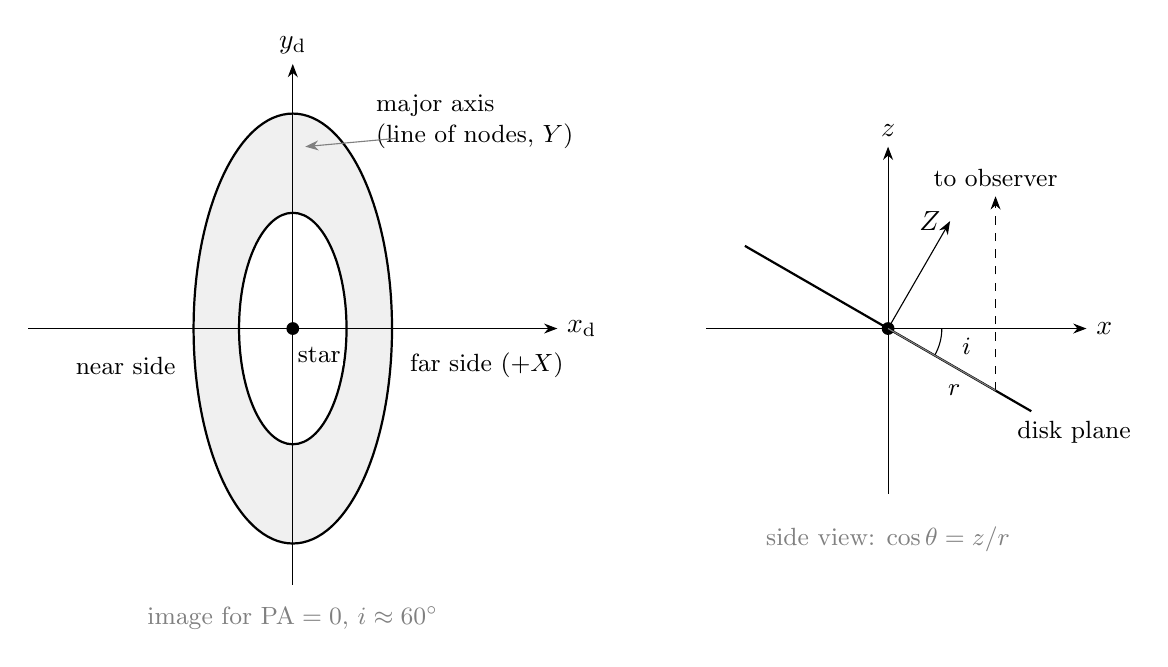
\begin{tikzpicture}[scale=1.05, >=Stealth]
  % disk ellipse
  \draw[thick, fill=gray!12] (0,0) ellipse (1.2 and 2.6);
  \draw[thick, fill=white] (0,0) ellipse (0.65 and 1.4);
  \fill (0,0) circle (2.2pt);
  \node[font=\small, fill=white, inner sep=1pt] at (0.32,-0.32) {star};
  % detector axes
  \draw[->] (-3.2,0) -- (3.2,0) node[right] {$x_\mathrm{d}$};
  \draw[->] (0,-3.1) -- (0,3.2) node[above] {$y_\mathrm{d}$};
  % labels
  \node[align=left, font=\small] at (2.2,2.5) {major axis\\(line of nodes, $Y$)};
  \draw[->, gray] (1.25,2.3) -- (0.15,2.2);
  \node[font=\small, anchor=east] at (-1.3,-0.45) {near side};
  \node[font=\small, anchor=west] at (1.3,-0.45) {far side ($+X$)};
  \node[font=\small, gray] at (0,-3.5) {image for $\mathrm{PA}=0$, $i\approx 60^\circ$};
  % right panel: side view
  \begin{scope}[xshift=7.2cm]
    \draw[->] (-2.2,0) -- (2.4,0) node[right] {$x$};
    \draw[->] (0,-2.0) -- (0,2.2) node[above] {$z$};
    \draw[thick, rotate=-30] (-2.0,0) -- (2.0,0);
    \node[font=\small] at (2.25,-1.25) {disk plane};
    \draw[->, rotate=-30] (0,0) -- (0,1.5) node[left] {$Z$};
    \draw (0.65,0) arc (0:-30:0.65);
    \node[font=\small] at (0.95,-0.22) {$i$};
    \fill (0,0) circle (2.2pt);
    \draw[dashed,->] (1.3,-0.75) -- (1.3,1.6) node[above, font=\small] {to observer};
    \draw[gray] (0,0) -- (1.3,-0.75);
    \node[font=\small] at (0.8,-0.75) {$r$};
    \node[font=\small, gray] at (0,-2.55) {side view: $\cos\theta = z/r$};
  \end{scope}
\end{tikzpicture}
\caption{Left: the detector frame and the projected disk. Right: the disk plane seen from the
side; the scattering angle $\theta$ of a grain is the angle between the direction from the star
to the grain and the direction to the observer.}
\label{fig:frames}
\end{figure}

\subsection{Radial density laws}

The disk consists of $N_\mathrm{b}\le 10$ belts. Belt $k$ has a radial law $n_k(\mathcal{A})$,
where $\mathcal{A}$ is the semi-major axis of the orbit through a point (for circular belts
$\mathcal{A}$ is the distance from the star). The built-in laws are
\begin{align}
\text{power law:}\quad & n(\mathcal{A}) \propto (\mathcal{A}/\mathrm{au})^{-\alpha},
  \label{eq:pl}\\
\text{Ertel peak:}\quad & n(\mathcal{A}) \propto s^{\alpha}\exp[\alpha(1-s)],\quad
  s = \frac{\mathcal{A}-R_\mathrm{start}}{R_\mathrm{peak}-R_\mathrm{start}},\quad
  n = 0 \text{ for } \mathcal{A}<R_\mathrm{start},\\
\text{Gaussian:}\quad & n(\mathcal{A}) \propto (\mathcal{A}/\mathrm{au})^{\alpha}
  \exp\!\left[-\tfrac{1}{2}\left(\tfrac{\mathcal{A}-\mu}{\sigma}\right)^2\right],\\
\text{broken power law:}\quad & n(\mathcal{A}) \propto
  \left[(\mathcal{A}/R_\mathrm{c})^{-2\alpha_\mathrm{in}} +
        (\mathcal{A}/R_\mathrm{c})^{-2\alpha_\mathrm{out}}\right]^{-1/2},
  \label{eq:broken}
\end{align}
with $\alpha_\mathrm{in}>0$ and $\alpha_\mathrm{out}<0$ for the broken power law (Augereau et
al.\ 1999). The law is evaluated only for $R_\mathrm{in}\le\mathcal{A}\le R_\mathrm{out}$; outside
it the density is zero. A fifth law calls the function \code{user\_density\_fn} in
\code{src/user\_density.f90} (Sect.~\ref{sec:extend}). It receives $\mathcal{A}$, the disk-frame
coordinates and ten free parameters, so azimuthal clumps, arcs, spirals or gaps can be modelled
without changing the rest of the code.

\subsection{Eccentric belts}
\label{sec:ecc}

The orbits of a belt are confocal (the star sits in one focus), share the eccentricity $e$ and
are aligned, with the argument of pericentre $\omega$ measured in the disk plane from $+Y$
towards $+X$. A point at distance $s$ from the star and azimuth $\psi=\operatorname{atan2}(X,Y)$
lies on the orbit with
\begin{equation}
\mathcal{A} = \frac{s\,[1+e\cos(\psi-\omega)]}{1-e^2}.
\label{eq:aorb}
\end{equation}
The particles are assumed to be spread uniformly in mean anomaly along each orbit. By Kepler's
second law a particle spends a time $\propto s^2$ per unit true anomaly, so for a given
$\mathcal{A}$ the number of particles per $\dd\mathcal{A}\,\dd\psi$ is proportional to $s^2$. At fixed azimuth,
$\partial s/\partial\mathcal{A}=s/\mathcal{A}$, so the area element is
$s\,\dd s\,\dd\psi=(s^2/\mathcal{A})\,\dd\mathcal{A}\,\dd\psi$. The factor $s^2$ cancels, and the
surface density depends on $\mathcal{A}$ alone. The local thickness of the disk is proportional
to the distance $s$ for both vertical profiles below, so the volume density is
\begin{equation}
\rho(s,\psi) = n(\mathcal{A})\,\frac{\mathcal{A}}{s},
\label{eq:eccdens}
\end{equation}
which reduces to $n(s)$ for $e=0$. The dust extends from the pericentre
$R_\mathrm{in}(1-e)$ to the apocentre $R_\mathrm{out}(1+e)$. The grain temperatures follow the true
distance. At a given $\mathcal{A}$ the surface density is the same at pericentre and apocentre and
the dust at pericentre is warmer, so in a face-on image that resolves the width of the ring the
surface brightness is highest at pericentre at all wavelengths (pericentre glow). The ring is
wider at apocentre, by the factor $(1+e)/(1-e)$ for a belt with sharp edges, and therefore holds
more dust per unit length along the ring. In the flux integrated across the ring this outweighs
the lower temperature at millimetre wavelengths, where the emission depends only weakly on
temperature: in the Rayleigh--Jeans limit the apocentre is brighter by $[(1+e)/(1-e)]^{1/2}
\approx 1+e$ (apocentre glow; Pan et al.\ 2016). The same holds in images whose beam is wider
than the ring. For the images of \code{examples/eccentric\_ring.nml} ($e=0.3$, face-on) the
apocentre-to-pericentre ratio is 1.27 for the 870\um\ flux per unit length (summed over
$\pm5^\circ$ in azimuth around each apsis) and 0.69 for the peak surface brightness; at 24\um\ the
two ratios are 0.23 and 0.12.

\subsection{Vertical structure}

All belts share one vertical structure:
\begin{itemize}
\item \textbf{Wedge.} $\rho = n(\mathcal{A})\,\mathcal{A}/s$ inside $|Z|\le s\sin\vartheta$, where
      $s=r$ is the 3-d distance and $\vartheta$ the half opening angle; zero outside.
\item \textbf{Gaussian.} $\rho = n(\mathcal{A})\,(\mathcal{A}/\varpi)\exp(-Z^2/2h^2)$ with
      $h=(h/r)\,\varpi$; here $s=\varpi$ is the distance in the disk plane and the radial law gives
      the mid-plane density. The profile is cut at $|Z| = c\,h$ ($c=4$ by default).
\end{itemize}

\subsection{Several belts}

The amplitude of each belt is set so that belt $k$ holds the fraction $f_k$ of the dust mass that
survives sublimation and blow-out (Sect.~\ref{sec:subl}):
\begin{equation}
M_k = \int \rho_k(\mathbf{x})\,\mu(r)\,\dd V,\qquad A_k \propto \frac{f_k}{M_k},
\end{equation}
where $\mu(r)$ is the surviving mass fraction at distance $r$. The integral is evaluated in
spherical disk coordinates with 800 logarithmic radial cells, 48 latitude cells and 360 azimuth
cells. Inclination, position angle and vertical structure are common to all belts.

%----------------------------------------------------------------------------------------------------
\section{The star}
\label{sec:star}

The stellar surface intensity $I_{\star,\lambda}$ comes from one of three sources:
\begin{enumerate}
\item a black body, $I_{\star,\lambda}=B_\lambda(T_\mathrm{eff})$;
\item an observed or model spectrum $F_{\nu}$ in Jy at the distance $d$, converted to
      $I_{\star,\lambda} = F_\nu\,(c/\lambda^2)\,d^2/(\pi R_\star^2)$;
\item a model-atmosphere grid: two columns, wavelength and surface flux
      $F_\lambda=\pi I_{\star,\lambda}$, for a set of $(T_\mathrm{eff},\log g)$. \dms\ interpolates
      bilinearly in $(T_\mathrm{eff},\log g)$ in $\log F_\lambda$ on the wavelength grid of the
      first model used.
\end{enumerate}
Longward of the last tabulated wavelength of a spectrum, a Rayleigh--Jeans continuation is used;
shortward of the first one the intensity is set to zero.
The luminosity is $L_\star = 4\pi^2R_\star^2\int I_{\star,\lambda}\,\dd\lambda$, and the flux at
distance $r$ from the star is $F_{\star,\lambda}(r)=\pi I_{\star,\lambda}R_\star^2/r^2$. The
stellar mass enters only through the blow-out size.

%----------------------------------------------------------------------------------------------------
\section{Dust grains}
\label{sec:grains}

\subsection{Size distribution}

The grain radii are binned logarithmically between $a_\mathrm{min}$ and $a_\mathrm{max}$. For the
power law $\dd N \propto a^{-q}\,\dd a$, the weight of bin $j$ with edges $a_{j-1}$ and $a_j$ is
\begin{equation}
w_j = \int_{a_{j-1}}^{a_j} a^{-q}\,\dd a = \frac{a_j^{1-q}-a_{j-1}^{1-q}}{1-q}.
\end{equation}
A single size and a table read from a file (radius and relative number per bin) are also
possible. For a table, the bin edges are the geometric means of neighbouring radii. If there are
several components with relative abundances $X_c$, all components share the same size
distribution. $X_c$ is therefore the fraction of grains by number, which is also the fraction by
volume; the mass fractions follow from the bulk densities. The number of grains per kilogram of dust is
\begin{equation}
N_{jc} = \frac{X_c\,w_j}{\sum_{j',c'} X_{c'}\,w_{j'}\,m_{j'c'}},\qquad
m_{jc} = \tfrac{4}{3}\pi a_j^3\,\rho_{\mathrm{b},c}.
\end{equation}

\subsection{Composite grains: effective-medium theory}
\label{sec:emt}

A grain made of several materials can be described by an effective dielectric function
$\varepsilon_\mathrm{eff}$ (with $\varepsilon=m^2$) and then treated as a homogeneous sphere.
\dms\ has four rules built in, for an inclusion with volume fraction $f$ and dielectric function
$\varepsilon_i$ in a matrix $\varepsilon_m$:
\begin{align}
\text{Maxwell Garnett:}\quad & \varepsilon_\mathrm{eff} = \varepsilon_m
   \frac{\varepsilon_i+2\varepsilon_m+2f(\varepsilon_i-\varepsilon_m)}
        {\varepsilon_i+2\varepsilon_m-f(\varepsilon_i-\varepsilon_m)},\\
\text{Bruggeman:}\quad & f\,\frac{\varepsilon_i-\varepsilon_\mathrm{eff}}{\varepsilon_i+2\varepsilon_\mathrm{eff}}
   + (1-f)\,\frac{\varepsilon_m-\varepsilon_\mathrm{eff}}{\varepsilon_m+2\varepsilon_\mathrm{eff}} = 0,\\
\text{Lichtenecker:}\quad & \ln\varepsilon_\mathrm{eff} = f\ln\varepsilon_i + (1-f)\ln\varepsilon_m,\\
\text{Looyenga:}\quad & \varepsilon_\mathrm{eff}^{1/3} = f\,\varepsilon_i^{1/3} + (1-f)\,\varepsilon_m^{1/3}.
\end{align}
For more than two materials, non-spherical inclusions (needles, platelets) and coated grains, the
Python module \code{dms.emc} drives the code \code{emc} of Ossenkopf (1991), which is not part of
\dms\ and must be installed separately (Sect.~\ref{sec:emcuse}). The combinations used in the
water-ice studies are listed in Table~\ref{tab:emc}.

\begin{table}[h]
\centering
\caption{Combinations of \code{emc} theories and inclusion shapes used in our water-ice studies.
\code{dms.emc} accepts any combination of the theories and shapes listed in
Sect.~\ref{sec:emcuse}.}
\label{tab:emc}
\small
\begin{tabularx}{\textwidth}{@{}R{5.2cm}R{4.0cm}X@{}}
\toprule
Label & Theory & Shape of the inclusions \\
\midrule
MG sphere, MG needle, MG platelet & Maxwell Garnett & sphere, needle, platelet \\
BG sphere & Bruggeman & sphere \\
BG needle, BG platelet & Bruggeman & needle or platelet (ice), sphere (refractory) \\
UniMG coated, UniBG coated & universal MG, universal BG & refractory core coated with ice \\
\bottomrule
\end{tabularx}
\end{table}

All four rules assume inclusions much smaller than the wavelength. Maxwell Garnett treats matrix
and inclusion differently and is meant for dilute inclusions; Bruggeman treats all components
alike.

\paragraph{Porosity.} Porous grains are mixtures with vacuum ($\varepsilon=1$) as one component.
\paragraph{Internal and external mixing.} In an internal mixture each grain contains all materials
and has one effective dielectric function. In an external mixture each material forms its own
grains; \dms\ treats every material as a separate component with its own abundance, temperature
and blow-out size.
\paragraph{Bulk density.} The bulk density of every component is an input. For an internal
mixture it is the volume-weighted mean, $\rho_\mathrm{b}=\sum_j f_j\rho_{\mathrm{b},j}$, with
vacuum counted as zero; \dms\ does not compute it.

\subsection{Distribution of hollow spheres}
\label{sec:dhs}

Irregular grains can be approximated by a distribution of hollow spheres (DHS; Min et al.\ 2005).
The vacuum volume fraction $f$ of the central cavity is uniformly distributed between 0 and
$f_\mathrm{max}$. The material volume, and therefore the mass, is that of a solid sphere of radius
$a$; the outer and inner radii are
\begin{equation}
a_\mathrm{out} = a\,(1-f)^{-1/3},\qquad a_\mathrm{core} = a\,(1-f)^{-1/3}f^{1/3}.
\end{equation}
Cross sections and scattering-matrix elements are averaged over $f$ with $n_f$ Gauss--Legendre
points; $S_{11}$ and $S_{12}$ are weighted with $C_\mathrm{sca}$. Efficiencies refer to $\pi a^2$.
The coated-sphere coefficients are computed with the algorithm of Yang (2003), as used by Pe\~na \&
Pal (2009). The downward recurrences start at $1.07\max(n_\mathrm{max},|mx|)+30$; with a margin of
only about 16 terms, large and nearly non-absorbing spheres were wrong by up to 0.1\,per cent.
Min et al.\ (2005) took $f_\mathrm{max}=1$,
the most extreme shape distribution, as their default and compared $f_\mathrm{max}=0.3$--0.5 with
laboratory measurements of quartz; Min et al.\ (2016) adopted $f_\mathrm{max}=0.8$. \dms\ accepts
$0<f_\mathrm{max}\le1$ (default 0.8) and $1\le n_f\le100$ (default 10); with $n_f=10$ and
$f_\mathrm{max}=1$ the largest node is $f=0.987$. The DHS
step is 10--20 times slower than the Mie step for compact spheres.

%----------------------------------------------------------------------------------------------------
\section{Optical properties}
\label{sec:optics}

\subsection{Mie theory and wavelength grids}

Optical data files give $n_\mathrm{r}$ and $k$ against wavelength. \dms\ uses two wavelength
grids.
\begin{itemize}
\item The \emph{internal grid} is the union of the wavelengths of all optical-data files within the
      range that all files cover; every data set is interpolated onto it, linearly in
      $\log\lambda$. The order of the components therefore does not matter. On this grid \dms\
      computes $Q_\mathrm{abs}$ and $Q_\mathrm{pr}$, which enter the temperatures and the radiation
      pressure.
\item The \emph{observing wavelengths} are given by the user. At these wavelengths \dms\ repeats the Mie
      calculation with the refractive index interpolated to each observing wavelength, which is
      more accurate than interpolating the efficiencies, in particular inside absorption bands.
\end{itemize}
The Mie routine is \code{miex} (Wolf \& Voshchinnikov 2004), which was written for very large
size parameters. For \dms\ 2.0 its work array is allocated with the number of terms actually
needed, and it keeps no saved variables, so it can be called from OpenMP threads.

\subsection{Scattering matrix}

For every grain size, material and observing wavelength, \dms\ stores
$C_\mathrm{abs}$, $C_\mathrm{sca}$ and the normalised matrix elements
\begin{equation}
\hat S_{11}(\theta) = \frac{S_{11}(\theta)}{k^2C_\mathrm{sca}},\qquad
\hat S_{12}(\theta) = \frac{S_{12}(\theta)}{k^2C_\mathrm{sca}},\qquad
\int_{4\pi}\hat S_{11}\,\dd\Omega = 1,
\end{equation}
with $k=2\pi/\lambda$ (Bohren \& Huffman 1983), on $N_\theta$ equidistant angles between
$0^\circ$ and $180^\circ$ (181 by default). The degree of linear polarisation of light scattered by
one grain is $-S_{12}/S_{11}$; it is positive for polarisation perpendicular to the scattering
plane, where $S_{12}<0$.

\paragraph{Forward-scattering peak.} \dms\ interpolates $\hat S_{11}$ and $\hat S_{12}$ linearly
in $\theta$ between the grid angles. For large grains the forward diffraction peak (width
$\approx1/x$\,rad, $x=2\pi a/\lambda$) and the first diffraction rings are much narrower than the
angle step, and interpolating point values there would put far too much light at small
scattering angles, i.e.\ into edge-on disks and lines of sight close to the star. \dms\ therefore
\begin{enumerate}
\item averages $\hat S_{11}$ and $\hat S_{12}$ over the angle bin of each grid angle in the forward
      region ($\theta\lesssim30/x$), computed from the Mie coefficients with at least four samples
      per ring period;
\item normalises $\int\hat S_{11}\,\dd\Omega=1$ with the exact weights of the linear interpolation
      used in the integration, by rescaling $\hat S_{11}$ and $\hat S_{12}$ only in the forward
      region $\theta<6/x$ (at least the first three grid angles), where the energy missed by the grid
      lies; for small grains and Henyey--Greenstein functions this region is the whole sphere;
\item refines volume elements (images) and integration cells (SED) close to the forward direction
      (Sect.~\ref{sec:amr}).
\end{enumerate}
Beyond the forward region the values at the grid angles are used. Section~\ref{sec:verify} gives
the accuracy reached.

\subsection{Henyey--Greenstein phase functions}

Instead of Mie theory, the phase function can be a one- or two-component Henyey--Greenstein
function,
\begin{equation}
p(\theta) = w\,\mathrm{HG}(g_1,\theta) + (1-w)\,\mathrm{HG}(g_2,\theta),\qquad
\mathrm{HG}(g,\theta) = \frac{1}{4\pi}\frac{1-g^2}{(1+g^2-2g\cos\theta)^{3/2}},
\end{equation}
with a Rayleigh-like degree of polarisation
\begin{equation}
P(\theta) = -p_\mathrm{max}\,\frac{\sin^2\theta}{1+\cos^2\theta},\qquad
\hat S_{12} = P\,p(\theta).
\end{equation}
This Rayleigh-like dependence of the polarisation on the scattering angle was used, for example,
by Engler et al.\ (2017). The cross sections $C_\mathrm{abs}$ and $C_\mathrm{sca}$ still come from
Mie theory.

\subsection{Radiation pressure and blow-out}
\label{sec:beta}

The ratio of radiation pressure to gravity is (Burns et al.\ 1979)
\begin{equation}
\beta(a) = \frac{3L_\star\,\langle Q_\mathrm{pr}\rangle_\star}{16\pi G M_\star c\,\rho_\mathrm{b}\,a},
\qquad
\langle Q_\mathrm{pr}\rangle_\star = \frac{\int Q_\mathrm{pr}(a,\lambda)\,I_{\star,\lambda}\,\dd\lambda}
                                         {\int I_{\star,\lambda}\,\dd\lambda},
\end{equation}
with $Q_\mathrm{pr}=Q_\mathrm{ext}-g\,Q_\mathrm{sca}$, where $g=\langle\cos\theta\rangle$ is the
asymmetry parameter.

A grain released at distance $r$ from a parent body on an orbit with semi-major axis $\mathcal{A}$
has the parent's velocity, but feels the stellar gravity reduced by the factor $1-\beta$. Its orbit
is unbound if
\begin{equation}
\beta \ge \beta_\mathrm{crit} = \frac{r}{2\mathcal{A}} = \frac{1-e^2}{2\,(1+e\cos f)},
\label{eq:betacrit}
\end{equation}
where $f$ is the true anomaly of the release point: $\beta_\mathrm{crit}=1/2$ for circular orbits,
$(1-e)/2$ for release at pericentre and $(1+e)/2$ for release at apocentre. With
\code{blowout = .true.}, grains with $\beta\ge\beta_\mathrm{crit}$ are removed. The input
\code{blowout\_release} selects $\beta_\mathrm{crit}$: \code{'circular'} (1/2, the default),
\code{'pericentre'} or \code{'apocentre'}, using the eccentricity of each belt; \code{blowout\_beta}
sets any other value. The population of grains in \dms\ depends on the distance from the star, not
on the azimuth, so $\beta_\mathrm{crit}$ is applied per distance: within the distance range of a
belt its value is used, where belts overlap the smaller value applies, and the smallest and largest
value are reported (summary, FITS keywords \code{BETACMIN} and \code{BETACMAX},
\code{Result.blowout\_beta}). Because $\langle Q_\mathrm{pr}\rangle_\star$ depends on the composition and on the stellar
spectrum, the blow-out size differs between materials and stars. It is computed for every
component, after sublimation and with the temperature-dependent optical data if these are used.

%----------------------------------------------------------------------------------------------------
\section{Temperatures and sublimation}
\label{sec:temp}

\subsection{Radiative equilibrium}

A grain of radius $a$ at distance $r$ absorbs
$\int C_\mathrm{abs}\,\pi I_{\star,\lambda}R_\star^2/r^2\,\dd\lambda$ and emits
$4\pi\int C_\mathrm{abs}B_\lambda(T)\,\dd\lambda$. Equating the two gives the distance at which a
grain has temperature $T$:
\begin{equation}
r(T) = \frac{R_\star}{2}\left[\frac{\int C_\mathrm{abs}(a,\lambda)\,I_{\star,\lambda}\,\dd\lambda}
                                     {\int C_\mathrm{abs}(a,\lambda)\,B_\lambda(T)\,\dd\lambda}\right]^{1/2}.
\label{eq:rT}
\end{equation}
For a black-body grain around a black-body star this gives the familiar
$T=T_\mathrm{eff}\,(R_\star/2r)^{1/2}$. \dms\ evaluates Eq.~(\ref{eq:rT}) on a table of
temperatures for every grain size and material, makes $r(T)$ monotonic, and interpolates
$\log r$ to obtain $T(r)$ on a logarithmic distance grid that covers all dust. The factor
$R_\star^2/4r^2$ assumes that the star appears as a point; within a few stellar radii the dilution
factor of an extended star would be needed.

\subsection{Temperature-dependent optical constants}

For one component, optical data can be given at several temperatures (e.g.\ crystalline water
ice). Each grain uses the data set closest to its own temperature, at all wavelengths.

\subsection{Sublimation}
\label{sec:subl}

Each component can have a sublimation temperature $T_\mathrm{s}$. Where a grain is hotter than
$T_\mathrm{s}$, it either disappears or turns into another component (the \emph{residue}); for
example, ice--silicate grains become porous silicate grains (Kim et al.\ 2019). The components are
processed in order of increasing $T_\mathrm{s}$, so a residue can itself sublimate further in.
Sublimation and blow-out together define, at every distance, the number of grains of every size
and component per kilogram of initial dust and the surviving mass fraction $\mu(r)$. The input
dust mass refers to the surviving grains.

%----------------------------------------------------------------------------------------------------
\section{Emission, scattering and polarisation}
\label{sec:rad}

\subsection{Contribution of one volume element}

Consider a volume element $\dd V$ at position $\mathbf{x}$, distance $r$ from the star, containing
the dust mass $\dd m=\rho\,\dd V$. With $N_{jc}(r)$ grains of size $j$ and component $c$ per unit
mass, the flux densities received at distance $d$ are
\begin{align}
\dd F^\mathrm{th}_\lambda &= \frac{\dd m}{d^2}\sum_{j,c} N_{jc}\,C^\mathrm{abs}_{jc}(\lambda)\,
                             B_\lambda\!\left(T_{jc}(r)\right), \label{eq:th}\\
\dd F^\mathrm{sca}_\lambda &= \frac{\dd m}{d^2}\sum_{j,c} N_{jc}\,C^\mathrm{sca}_{jc}(\lambda)\,
                             \hat S_{11,jc}(\lambda,\theta)\,\frac{\pi I_{\star,\lambda}R_\star^2}{r^2},
                             \label{eq:sca}\\
\dd P_\lambda &= \frac{\dd m}{d^2}\sum_{j,c} N_{jc}\,C^\mathrm{sca}_{jc}(\lambda)\,
                             \hat S_{12,jc}(\lambda,\theta)\,\frac{\pi I_{\star,\lambda}R_\star^2}{r^2},
                             \label{eq:pol}
\end{align}
with the scattering angle $\cos\theta=z/r$ (observer at $+z$). The sums are tabulated before the
integration as kernels per kilogram of dust at every distance of the distance grid, and $\hat
S_{11}$, $\hat S_{12}$ are interpolated linearly in $\theta$. Flux densities per unit wavelength
are converted to Jy with $F_\nu=F_\lambda\lambda^2/c$.

\subsection{Stokes parameters}

$\dd P_\lambda<0$ means polarisation perpendicular to the scattering plane. With
$\phi=\operatorname{atan2}(y_\mathrm{d},x_\mathrm{d})$, the Stokes parameters are
\begin{equation}
\dd Q = \dd P\cos2\phi,\qquad \dd U = \dd P\sin2\phi,
\end{equation}
so that $Q>0$ means polarisation along the image $x$ axis. The polarised intensity is
$\mathrm{PI}=\sqrt{Q^2+U^2}$, and the azimuthal Stokes parameters are
\begin{equation}
Q_\phi = -(Q\cos2\phi + U\sin2\phi),\qquad U_\phi = Q\sin2\phi - U\cos2\phi .
\end{equation}
For optically thin single scattering the polarisation is perpendicular to the direction to the
star, so $Q_\phi>0$ and $U_\phi\approx0$. Observers often count $\phi$ from north through east;
the sign of $Q_\phi$ is the same in that convention, while $U_\phi$ may change sign. The degree of
polarisation is $\mathrm{PI}/I$, where $I$ is the dust intensity (thermal plus scattered, without
the star).

\subsection{Global quantities}

\begin{itemize}
\item \textbf{Fractional luminosity:}
      $f_\mathrm{d} = \sum N\pi a^2\langle Q_\mathrm{abs}\rangle_\star/(4\pi r^2)$, summed over
      all grains. It is accumulated during the integration. The integrated thermal SED
      reproduces it to better than 0.1\,per cent (Sect.~\ref{sec:verify}).
\item \textbf{Geometrical optical depth} ($Q_\mathrm{ext}=1$): along every line of sight
      (\code{image\_tau}); vertically, $\tau_\perp(\varpi)=\int n\pi a^2\,\dd Z$, as an azimuthal
      mean and towards pericentre and apocentre; and as the mean
      $\tau_\mathrm{mean}=\sum N\pi a^2/S$, with the disk area
      $S=\sum_k\pi(R_{\mathrm{out},k}^2-R_{\mathrm{in},k}^2)\sqrt{1-e_k^2}$.
\item \textbf{Mass scaling:} all quantities are first computed per unit density and then scaled
      so that the surviving dust mass equals the input dust mass.
\end{itemize}

%----------------------------------------------------------------------------------------------------
\section{Images and adaptive volume refinement}
\label{sec:amr}

\subsection{Image grid}

The image has $N\times N$ pixels ($N$ odd), with the star in the central pixel. The field covers
$\pm R_\mathrm{field}$, where $R_\mathrm{field}$ is the largest distance of dust from the star:
the apocentre of the outermost orbit for the wedge, and that distance divided by
$\cos\vartheta_\mathrm{cut}$ for the Gaussian profile, whose cut extends above the disk plane.
Along the line of sight through each pixel, the model space is divided into cubes of the pixel
size. Each cube is a \emph{volume element}; its contribution to the pixel is computed with
Eqs.~(\ref{eq:th})--(\ref{eq:pol}) at its centre.

\subsection{Why refinement is needed}

A volume element of one pixel can be much larger than the scales on which the integrand varies:
the disk edges, a thin disk seen edge-on, a narrow belt, or the steep temperature gradient close
to the star. Evaluating the integrand once per element would then misplace or miss flux. A finer
image grid everywhere would be expensive, since most elements contain either no dust or smoothly
varying dust. \dms\ therefore refines only where needed.

\subsection{Splitting criteria}

A volume element (cube of half size $h$) is split into eight sub-cubes of half size $h/2$, and the
test is repeated for each of them (an octree, Fig.~\ref{fig:amr}). A cube is \emph{not} split
further if all of the following hold:
\begin{enumerate}
\item \textbf{Temperature.} The temperature of the smallest grain of the first component, evaluated
      at the smallest and the largest distance of the cube from the star, differs by less than
      $\Delta T_\mathrm{max}$ (\code{max\_delta\_t}, 2\,K by default).
\item \textbf{Density.} The density at the eight corners and at the centre is either non-zero
      everywhere and smooth, $|(\rho_\mathrm{max}+\rho_\mathrm{min})/2-\rho_\mathrm{c}|\le0.01\,
      \rho_\mathrm{c}$, or zero everywhere. A cube that is zero at all nine points but thicker than
      the local disk thickness is still split, so that a thin disk cannot slip between the test
      points.
\end{enumerate}
The splitting level is limited by $N_\mathrm{max}$ (\code{n\_split\_max}, 3 by default), so that
a pixel-sized element is divided into at most $8^{N_\mathrm{max}}$ sub-cubes.

\paragraph{Refinement near the star.} Close to the star a volume element can be large compared
with its distance to the star, for example when dust extends to 0.01\,au in an image of
$\pm150$\,au. With the cap $N_\mathrm{max}$ alone, the warm inner dust is then under-sampled. In
\dms\ 2.0 the splitting continues beyond $N_\mathrm{max}$ (temperature and boundary criteria only) as long as
the cube is larger than $0.05$ times its distance to the star, $2h>0.05\max(r_\mathrm{min},
R_\mathrm{in,eff})$, up to an absolute limit of 30 levels. Elsewhere $N_\mathrm{max}$ applies as
before.

\paragraph{Refinement near the forward direction and in narrow belts.} When scattered light is
computed, elements whose scattering angle lies within two angle-grid steps of the forward
direction are split, also beyond $N_\mathrm{max}$, until their angular size seen from the star is
below a quarter of the grid step and they are smaller than half the width of the narrowest belt.
In addition, an element that overlaps a belt and has zero density at all nine test points is split
while it is wider than half the belt width, so that a belt narrower than an element cannot fall
between the test points.

\begin{figure}[t]
\centering
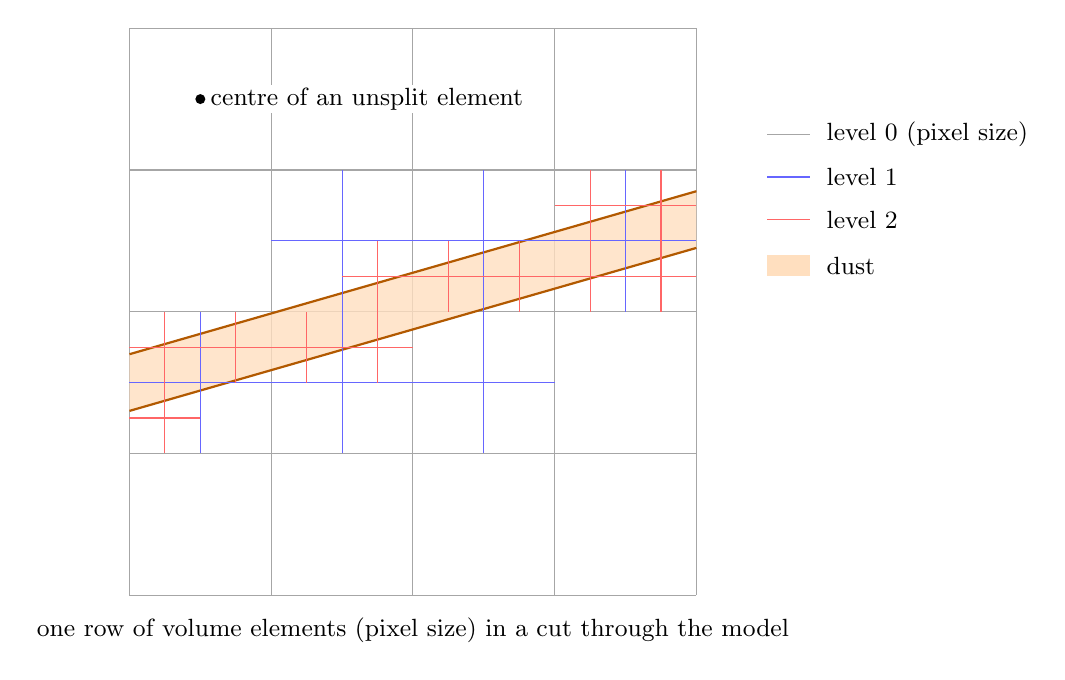
\begin{tikzpicture}[scale=0.9]
  % base grid 4x4 cells of size 2
  \foreach \i in {0,...,4} {
    \draw[gray!70] (\i*2,0) -- (\i*2,8);
    \draw[gray!70] (0,\i*2) -- (8,\i*2);
  }
  % disk band
  \fill[orange!25, opacity=0.8] (0,2.6) -- (8,4.9) -- (8,5.7) -- (0,3.4) -- cycle;
  \draw[orange!70!black, thick] (0,2.6) -- (8,4.9);
  \draw[orange!70!black, thick] (0,3.4) -- (8,5.7);
  % level 1 splits on cells crossing edges
  \foreach \x/\y in {0/2,2/2,2/4,4/2,4/4,6/4} {
    \draw[blue!60] (\x+1,\y) -- (\x+1,\y+2);
    \draw[blue!60] (\x,\y+1) -- (\x+2,\y+1);
  }
  % level 2 splits in some subcells
  \foreach \x/\y in {0/2,0/3,1/3,2/3,3/3,3/4,4/4,5/4,6/4,7/4,6/5,7/5} {
    \draw[red!60] (\x+0.5,\y) -- (\x+0.5,\y+1);
    \draw[red!60] (\x,\y+0.5) -- (\x+1,\y+0.5);
  }
  \fill (1,7) circle (2pt);
  \node[font=\small, right, fill=white, inner sep=1pt] at (1.1,7) {centre of an unsplit element};
  \node[font=\small] at (4,-0.5) {one row of volume elements (pixel size) in a cut through the model};
  % legend
  \begin{scope}[xshift=9cm, yshift=4.5cm]
    \draw[gray!70] (0,2) -- (0.6,2); \node[right,font=\small] at (0.7,2) {level 0 (pixel size)};
    \draw[blue!60] (0,1.4) -- (0.6,1.4); \node[right,font=\small] at (0.7,1.4) {level 1};
    \draw[red!60] (0,0.8) -- (0.6,0.8); \node[right,font=\small] at (0.7,0.8) {level 2};
    \fill[orange!25] (0,0) rectangle (0.6,0.3); \node[right,font=\small] at (0.7,0.15) {dust};
  \end{scope}
\end{tikzpicture}
\caption{Adaptive refinement, shown in two dimensions (the code splits cubes into eight
sub-cubes). Elements crossing the edges of the dust distribution or a strong temperature gradient
are split; elements inside smooth dust or in empty space are evaluated once.}
\label{fig:amr}
\end{figure}

\subsection{Implementation}

\begin{itemize}
\item \textbf{Depth-first stack.} The sub-cubes are kept on a stack (at most seven pending entries
      per level), so the memory needed per thread is small and fixed.
\item \textbf{Rejection of empty space.} Elements whose distance range lies entirely inside the
      innermost pericentre or outside the largest dust distance are skipped without evaluation.
\item \textbf{Parallelisation.} Pixels are distributed over OpenMP threads; the routines called in
      the inner loop only read global data.
\item \textbf{Mirror symmetry.} If $\mathrm{PA}=0$ and every belt is symmetric under
      $Y\to-Y$ (circular, or eccentric with the pericentre on the minor axis; user densities only
      when declared symmetric), only half of the image is computed and mirrored.
\item \textbf{Diagnostics.} Before the integration, \dms\ prints the temperature difference of the
      smallest grains across the finest sub-volume at the inner edge,
      $T(R_\mathrm{in,eff})-T(R_\mathrm{in,eff}+\sqrt3\,\Delta/2^{N_\mathrm{max}})$, where $\Delta$ is
      the pixel size, and warns if it exceeds $\Delta T_\mathrm{max}$
      (\code{max\_temp\_diff\_cals}).
\end{itemize}

%----------------------------------------------------------------------------------------------------
\section{SEDs}
\label{sec:sed}

\dms\ obtains SEDs in two ways.
\begin{enumerate}
\item \textbf{Direct quadrature} (\code{mode = 'sed'}). The disk is integrated in spherical disk
      coordinates: 400 logarithmic radial cells between the innermost pericentre and the largest
      dust distance, 16 latitude cells within the opening angle for the wedge (48 for the
      Gaussian profile) and 180 azimuth cells, with additional refinement near the forward
      direction. Every cell centre is transformed to the detector frame, so the scattering angles
      and the polarisation are those of the actual inclination. Equations~(\ref{eq:th})--(\ref{eq:pol})
      are evaluated at the cell centres. This is fast and needs no image.
\item \textbf{Summed images} (\code{mode = 'both'}). The images are computed and their pixels
      summed. This is the natural choice when images are needed anyway.
\end{enumerate}
For the thermal SED of the test models the two methods agree within 0.07\,per cent
(Sect.~\ref{sec:verify}). The scattered-light and polarised SEDs depend on the inclination through
the phase function; the thermal SED does not.

%----------------------------------------------------------------------------------------------------
\section{Simulated observations}
\label{sec:obs}

If a PSF or a mask is requested, \dms\ writes a second set of images, \code{image\_*\_obs}.
\begin{itemize}
\item \textbf{PSF.} A normalised 2-d Gaussian truncated at $4\sigma$, with
      $\sigma=\mathrm{FWHM}/(2\sqrt{2\ln2})$. The FWHM is given per wavelength, or set by
      diffraction, $\mathrm{FWHM}=1.029\,\lambda/D$ for a telescope of diameter $D$. The
      convolution is separable and conserves flux, apart from flux leaving the field.
\item \textbf{Polarisation after convolution.} $Q$ and $U$ are convolved; $\mathrm{PI}$,
      $Q_\phi$, $U_\phi$ and the degree of polarisation are then derived from the convolved $Q$
      and $U$, as in an observation.
\item \textbf{Star.} With \code{add\_star}, the star sits in the central pixel of the total image
      before the convolution, so \code{image\_total\_obs} contains the stellar PSF.
\item \textbf{Mask.} Pixels within the mask radius are set to NaN. The mask has a sharp edge; its
      transmission profile and the coronagraphic suppression of the stellar halo are not modelled.
\item \textbf{Noise.} No noise is added; the images are noise-free model images.
\item \textbf{Units.} Images are kept in Jy\,pixel$^{-1}$ internally and written in
      Jy\,pixel$^{-1}$, mJy\,arcsec$^{-2}$ or Jy\,arcsec$^{-2}$.
\end{itemize}

%----------------------------------------------------------------------------------------------------
\section{Verification}
\label{sec:verify}

Table~\ref{tab:verify} summarises the tests made for version~2.0. All use the astronomical
silicate of Draine (2003) unless noted otherwise. The checks that run in about a minute are part of
the automated test suite (Sect.~\ref{sec:tests}); the others were made once for this release.

\begin{table}[h]
\centering
\caption{Verification tests of \dms\ 2.0.}
\label{tab:verify}
\small
\begin{tabularx}{\textwidth}{@{}p{4.6cm}X@{}}
\toprule
Test & Result \\
\midrule
Energy balance & Two eccentric belts, Gaussian profile: integrated thermal SED$/L_\star =
  1.0006\,f_\mathrm{d}$ \\
Image SED vs.\ direct quadrature & Two belts, Gaussian profile: agreement within 0.07\,per cent \\
Belt mass fractions & Input 5/95\,per cent; recovered 4.97/95.03\,per cent from $\tau_\perp$ \\
Size distribution from a file & Identical to the same power law ($f_\mathrm{d}$ and SED to $10^{-6}$) \\
Model-atmosphere grid & Black-body grid: identical to the black-body star on a grid node;
  0.7\,per cent difference in $L_\star$ between the 5500 and 6000\,K nodes, from the interpolation
  in $\log F_\lambda$ \\
PSF convolution & Gaussian PSF (FWHM $0.5''$) and a $0.3''$ mask, single ring: 0.088750 vs.\
  0.088755\,Jy at 70\um\ \\
Refinement near the star & Original 2019 test model (dust from 0.01\,au, 101 pixels, $N_\mathrm{max}=3$):
  thermal flux at 1/10/100\um\ before the fix $1.1\times10^{-30}$/0.20/7.44\,Jy, after
  1.39/12.5/8.03\,Jy; direct quadrature 1.37/12.7/8.06\,Jy \\
DHS, $f_\mathrm{max}\to0$ & Equal to compact Mie spheres within $10^{-5}$ \\
Coated spheres & Agree with \code{scattnlay} (Pe\~na \& Pal 2009) to $10^{-10}$ in $Q$ and
  $10^{-7}$ in $S_{11}$, $S_{12}$ for size parameters 0.5--$10^4$ \\
Forward scattering & Exact integration of the Mie phase function (single size, ring at 100\,au,
  $5^\circ$ opening angle, 1.6\um, $x=1$--3927, $i=60^\circ$ and $88^\circ$): SED within 1.5\,per cent
  (largest deviation for $x\approx40$ edge-on), images within 0.8\,per cent for rings 2\,au wide or
  wider, within 6\,per cent for a 0.1-au ring seen edge-on \\
Polarisation & Stokes $Q$, $U$ of an inclined, rotated ring within 1\,per cent of the analytic result \\
Several optical-data grids & External ice mixtures with astrosilicate, pyroxene and organics against
  an independent Mie code: within 0.5 percentage points in the degree of polarisation \\
Threads & 1 and 2 OpenMP threads differ by $2\times10^{-13}$ \\
Robustness & 31 input cases (edge cases and invalid input) under AddressSanitizer,
  UndefinedBehaviorSanitizer, \code{-fcheck=all} and floating-point traps: no memory errors or
  undefined behaviour \\
Input routes & Namelist, interactive questions and Python give identical results \\
Compilers & \code{gfortran} 10.5 and 13.3; \code{make debug} without warnings \\
\bottomrule
\end{tabularx}
\end{table}

\FloatBarrier
%----------------------------------------------------------------------------------------------------
\section{Limitations}
\label{sec:limits}

Besides the assumptions in Sect.~\ref{sec:assumptions}, the following points limit the use of \dms.
\begin{itemize}
\item \textbf{Blow-out in eccentric belts.} In a belt with eccentricity $e$ the blow-out threshold
      depends on where along the orbit a grain is released, between $(1-e)/2$ and $(1+e)/2$
      (Eq.~\ref{eq:betacrit}). \dms\ applies one threshold per distance
      (\code{blowout\_release}, \code{blowout\_beta}), not one that varies with the azimuth, and it
      does not follow the new orbits of bound grains released with $\beta<\beta_\mathrm{crit}$.
\item \textbf{One size distribution.} All belts share one size distribution, which changes with
      distance only through sublimation and blow-out. A component whose small and large grains
      are distributed differently, such as a halo of small grains on eccentric orbits, has to be
      computed in a separate run with its own size distribution; images and SEDs of optically thin
      components add.
\item \textbf{Effective-medium grains.} EMT is valid for inclusions much smaller than the
      wavelength. Large inclusions or aggregates need methods such as DDA or T-matrix codes.
\item \textbf{Simulated observations.} Gaussian PSFs only, a sharp-edged mask, no noise and no
      instrumental polarisation. Use the noise-free images as input to an instrument simulator for
      a full prediction.
\item \textbf{Optically thick regions.} \dms\ reports the line-of-sight optical depth
      (\code{image\_tau}) and the largest radial optical depth in the mid-plane, and warns if the
      latter exceeds 0.1. Where these approach unity the results are no longer valid.
\item \textbf{No extinction of the starlight.} In reality the light diffracted by grains in front of
      the star stays within $\approx1/x$\,rad of the star and comes with the extinction of the
      starlight. \dms\ computes neither, so for edge-on disks the scattered SED contains
      forward-scattered light that an observation would not separate from the star.
\end{itemize}

%====================================================================================================
\part{User guide}
%====================================================================================================

\section{Installation}
\label{sec:install}

\subsection{Requirements}

\begin{itemize}
\item A Fortran compiler that supports Fortran 2008. The source files are free-form Fortran
      (\code{.f90}); version 2.0 also uses a few features introduced in Fortran 2003 and 2008,
      such as \code{error stop}, \code{open(newunit=...)}, \code{execute\_command\_line} and the
      \code{block} construct, and the \code{Makefile} compiles with \code{-std=f2008}. Tested with
      \code{gfortran} 10.5 and 13.3. The \code{Makefile} also has settings for Intel \code{ifx},
      which has not been tested.
\item GNU \code{make}. OpenMP is used if the compiler supports it.
\item For the Python interface: Python 3.9 or later and NumPy 1.22 or later. With Python 3.12 or
      later, \code{numpy.f2py} also needs \code{meson} and \code{ninja}. \code{astropy} (FITS) and
      \code{matplotlib} (plots) are optional.
\item For composite grains with \code{dms.emc}: the \code{emc} executable (Ossenkopf 1991),
      installed separately.
\item For the test suite: \code{pytest}.
\end{itemize}

On macOS, \code{gfortran} is available through Homebrew (\code{brew install gcc}); on Debian or
Ubuntu, through \code{apt install gfortran}. On Windows, use the Windows Subsystem for Linux.

\subsection{Getting the code and building}

\begin{lstlisting}[style=sh]
git clone https://github.com/<account>/dms.git   # <account>: owner of the repository
cd dms
make                        # optimised build with OpenMP   -> bin/dms
make python                 # Python extension (f2py)       -> python/dms/_dms*.so
pip install -e python       # optional: "import dms" from anywhere
\end{lstlisting}

Other targets of the \code{Makefile}:

\begin{center}
\small
\begin{tabular}{@{}ll@{}}
\toprule
Target & Effect \\
\midrule
\code{make} & optimised program with OpenMP (\code{-O3 -march=native}) \\
\code{make debug} & run-time checks, floating-point traps, no optimisation \\
\code{make serial} & optimised, without OpenMP \\
\code{make python} & Python extension from the same library \code{build/libdms.a} \\
\code{make test} & build program and Python module, run the test suite \\
\code{make clean} & remove build products \\
\code{make FC=ifx OMP=-qopenmp} & build with the Intel compiler \\
\bottomrule
\end{tabular}
\end{center}

The option \code{-march=native} optimises for the machine that compiles the code. If the
program is copied to another machine, build it there, or set \code{OPT="-O3"}.

\subsection{Testing the installation}
\label{sec:tests}

\begin{lstlisting}[style=sh]
bin/dms examples/debris_ring.nml
python3 tools/quicklook.py results ring -o ring.png
\end{lstlisting}
The first command prints the progress and a summary, and writes the results to \code{results/}.
The second makes a figure with the images, the SED and the optical-depth profile.

\paragraph{Test suite.} With \code{pytest} installed (\code{pip install pytest}),
\begin{lstlisting}[style=sh]
make test                         # build everything, run the tests
python3 -m pytest tests -v        # the same, test by test
\end{lstlisting}
runs the test suite in \code{tests/} (34 tests, about one minute on two cores):
\begin{itemize}
\item \textbf{physical checks} with known answers: energy balance (integrated thermal SED $=
      f_\mathrm{d}L_\star$), thermal SED from images against the direct quadrature, belt mass
      fractions, a size distribution read from a file against the same power law, the Rayleigh limit
      and the Henyey--Greenstein polarisation law for a face-on ring, the rotation of the image with
      the position angle, forward scattering on the near side, the radial extent of an eccentric
      belt, and the proportionality of all fluxes to the dust mass;
\item \textbf{blow-out}: default threshold, release at pericentre and apocentre, user value,
      thresholds per belt, conflicting inputs;
\item \textbf{interface}: invalid input raises \code{dms.DMSError} without ending the session,
      repeated runs, namelist round trip, command-line program against Python, exit codes;
\item \textbf{regression}: the seven examples, reduced in size, against the reference values in
      \code{tests/reference/examples.json} (relative tolerance $10^{-4}$; differences between
      compilers and thread counts are at the level of $10^{-12}$).
\end{itemize}
After a change that alters results on purpose, regenerate the reference values with
\code{python3 tests/regression.py --write} and explain the change in \code{CHANGELOG.md}.

\paragraph{Continuous integration.} On GitHub, the workflow \code{.github/workflows/tests.yml} runs
on every push and pull request (Ubuntu, Python 3.10 and 3.12): a debug build runs one example with
run-time checks and floating-point traps, then the optimised program and the Python module are built
and the test suite runs. The result is shown on the repository page under \emph{Actions}.

%----------------------------------------------------------------------------------------------------
\section{Repository layout}
\label{sec:layout}

\begin{center}
\small
\begin{tabularx}{\textwidth}{@{}lX@{}}
\toprule
Path & Content \\
\midrule
\code{src/} & Fortran source: modules, routines and the main program \code{dms.f90} \\
\code{src/user\_density.f90} & user-defined density distribution (edit and recompile) \\
\code{python/} & Python package \code{dms} and the f2py interface \code{dms\_api.f90} \\
\code{examples/} & input files showing the main features, and two Python examples \\
\code{data/optical\_constants/} & optical constants (wavelength [\um], $n$, $k$) \\
\code{data/stellar\_models/} & model-atmosphere grids (built with \code{python -m dms.stellar}) \\
\code{docs/} & input reference, outputs, conventions, Python interface, this manual \\
\code{tests/} & test suite (pytest) and reference values of the examples \\
\code{tools/} & quick-look plots, optical-constant plots \\
\code{.github/workflows/} & continuous integration (build and tests on GitHub) \\
\code{results/}, \code{cache/} & created at run time (output files, saved optical properties) \\
\bottomrule
\end{tabularx}
\end{center}

All directories can be changed in the input file (\code{\&run}: \code{data\_dir},
\code{output\_dir}, \code{cache\_dir}). Relative paths are taken relative to the working
directory, so the simplest way is to run \dms\ from the repository root.

%----------------------------------------------------------------------------------------------------
\section{Running \dms}
\label{sec:run}

\subsection{Command line}

\begin{lstlisting}[style=sh]
bin/dms model.nml              # input file (recommended)
bin/dms                        # interactive questions
bin/dms < answers.txt          # interactive questions answered from a file
bin/dms --help
export OMP_NUM_THREADS=8       # number of threads
\end{lstlisting}

\subsection{What happens during a run}

Figure~\ref{fig:flow} shows the sequence of a run. After every step \dms\ checks an error flag;
on an error it prints a message and stops (command line) or returns to Python.

\begin{figure}[h]
\centering
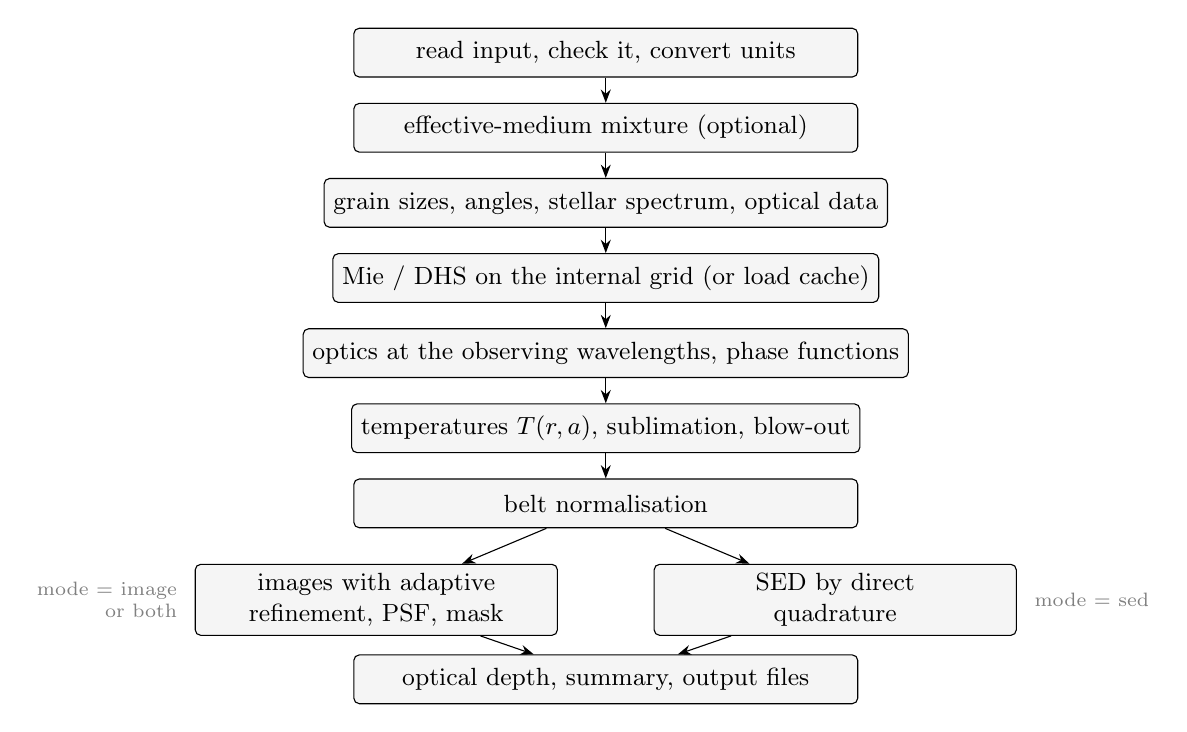
\begin{tikzpicture}[node distance=0.32cm, every node/.style={font=\small},
  box/.style={draw, rounded corners=2pt, fill=gray!8, minimum width=6.4cm, minimum height=0.62cm, align=center},
  >=Stealth]
  \node[box] (a) {read input, check it, convert units};
  \node[box, below=of a] (b) {effective-medium mixture (optional)};
  \node[box, below=of b] (c) {grain sizes, angles, stellar spectrum, optical data};
  \node[box, below=of c] (d) {Mie / DHS on the internal grid (or load cache)};
  \node[box, below=of d] (e) {optics at the observing wavelengths, phase functions};
  \node[box, below=of e] (f) {temperatures $T(r,a)$, sublimation, blow-out};
  \node[box, below=of f] (g) {belt normalisation};
  \node[box, below left=0.45cm and -2.6cm of g, minimum width=4.6cm] (h) {images with adaptive\\refinement, PSF, mask};
  \node[box, below right=0.45cm and -2.6cm of g, minimum width=4.6cm] (i) {SED by direct\\quadrature};
  \node[box, below=1.6cm of g] (j) {optical depth, summary, output files};
  \foreach \u/\v in {a/b,b/c,c/d,d/e,e/f,f/g} \draw[->] (\u) -- (\v);
  \draw[->] (g) -- (h); \draw[->] (g) -- (i);
  \draw[->] (h) -- (j); \draw[->] (i) -- (j);
  \node[right=0.2cm of h.east, xshift=-0.1cm, yshift=0.55cm, font=\scriptsize, gray] {};
  \node[left=0.1cm of h, font=\scriptsize, gray, align=right] {mode = image\\or both};
  \node[right=0.1cm of i, font=\scriptsize, gray, align=left] {mode = sed};
\end{tikzpicture}
\caption{Sequence of a run (\code{src/dms\_driver.f90}).}
\label{fig:flow}
\end{figure}

\subsection{A typical workflow}

\begin{enumerate}
\item Start from the example closest to your problem and copy it.
\item Set the star, the disk and the dust. Choose the observing wavelengths inside the wavelength
      range of the optical data.
\item Run \code{mode = 'sed'} first: it is fast and checks $f_\mathrm{d}$ and the SED.
\item Switch on images with a small image (e.g.\ 101 pixels), check them with
      \code{tools/quicklook.py}, then increase the resolution.
\item Save the optical properties (\code{save\_optics}) and reuse them
      (\code{load\_optics}) while you vary the geometry or the star.
\end{enumerate}

%----------------------------------------------------------------------------------------------------
\section{Input reference}
\label{sec:input}

An input file is a Fortran namelist with seven groups: \code{\&run}, \code{\&star}, \code{\&disk},
\code{\&image}, \code{\&wavelengths}, \code{\&dust} and \code{\&scattering}. All groups are optional
and may come in any order; a parameter that is not given keeps its default. Comments start with
\code{!}; strings are written in quotes, logicals as \code{.true.}/\code{.false.}, and lists are
separated by commas.

\textbf{Units:} lengths in au, angles in degrees, masses in $\Msun$, stellar radius in
$R_\odot$, distance in pc, grain radii and wavelengths in \um, temperatures in K.

\subsection{\code{\&run}: what to compute and where to write it}

\small
\begin{longtable}{@{}R{4.15cm}R{3.4cm}R{7.45cm}@{}}
\toprule
Name & Default & Meaning \\
\midrule
\endhead
\code{mode} & \code{'image'} & \code{'image'}; \code{'sed'} (direct integration, no images);
  \code{'both'} (images plus an SED from the summed images) \\
\code{emission} & \code{'both'} & \code{'thermal'}, \code{'scattering'}, \code{'both'},
  \code{'polarisation'} \\
\code{output\_format} & \code{'fits'} & \code{'ascii'}, \code{'fits'}, \code{'both'} (images) \\
\code{output\_name} & \code{''} & appended to all output file names \\
\code{name\_with\_parameters} & \code{.false.} & also append main model parameters to file names \\
\code{data\_dir} & \code{'data/}\allowbreak\code{optical\_constants/'} & directory of the optical data \\
\code{output\_dir} & \code{'results/'} & output directory (created if missing) \\
\code{cache\_dir} & \code{'cache/'} & directory of saved optical properties \\
\code{load\_optics} & \code{.false.} & reuse saved optical properties if radii, wavelengths, angles,
  grain shape and $n,k$ are identical \\
\code{save\_optics} & \code{.false.} & save the optical properties \\
\code{optics\_cache\_name} & \code{'dms\_optics'} & cache file name (in \code{dms.batch},
  \code{'auto'} derives it from the dust, wavelength and angle parameters) \\
\code{save\_temperature} & \code{.true.} & write the temperature distribution \\
\code{save\_grain\_sizes} & \code{.true.} & write grain numbers, cross sections and $\beta$ \\
\code{screen\_output} & \code{.true.} & print progress \\
\code{write\_files} & \code{.true.} & write output files (Python sets \code{.false.} by default) \\
\bottomrule
\end{longtable}
\normalsize

\subsection{\code{\&star}}

\small
\begin{longtable}{@{}R{4.15cm}R{3.4cm}R{7.45cm}@{}}
\toprule
Name & Default & Meaning \\
\midrule
\endhead
\code{spectrum} & \code{'blackbody'} & \code{'blackbody'}, \code{'file'}, \code{'grid'} \\
\code{teff} & 5800 & effective temperature [K] (black body or grid) \\
\code{logg} & 4.5 & $\log g$ [cgs] (grid) \\
\code{radius} & 1.0 & stellar radius [$R_\odot$] \\
\code{mass} & 1.0 & stellar mass [$\Msun$] (blow-out size) \\
\code{distance} & 10.0 & distance [pc] \\
\code{spectrum\_file} & & two columns: wavelength [\um], flux density [Jy] at \code{distance} \\
\code{grid\_dir} & & directory with \code{grid\_index.txt} (Sect.~\ref{sec:grids}) \\
\bottomrule
\end{longtable}
\normalsize

\subsection{\code{\&disk}}

Parameters marked \emph{per belt} are lists with one value per belt.

\small
\begin{longtable}{@{}R{4.15cm}R{3.4cm}R{7.45cm}@{}}
\toprule
Name & Default & Meaning \\
\midrule
\endhead
\code{n\_belts} & 1 & number of belts (at most 10) \\
\code{density\_law} & \code{'powerlaw'} & per belt: \code{'powerlaw'}, \code{'ertel'},
  \code{'gaussian'}, \code{'broken'}, \code{'user'} \\
\code{r\_in}, \code{r\_out} & required & per belt: inner and outer semi-major axis [au] \\
\code{eccentricity} & 0 & per belt: $0\le e<1$ \\
\code{omega} & 0 & per belt: argument of pericentre [deg], from the line of nodes ($+Y$) towards
  the far side ($+X$) \\
\code{belt\_mass\_fraction} & 1 & per belt: relative dust mass (normalised) \\
\code{alpha} & 1.0 & per belt: exponent of the radial law \\
\code{alpha\_out} & $-3.0$ & per belt: outer exponent (\code{'broken'}) \\
\code{r\_c} & & per belt: characteristic radius [au] (\code{'broken'}) \\
\code{r\_start}, \code{r\_peak} & & per belt [au] (\code{'ertel'}) \\
\code{mu}, \code{sigma} & & per belt: centre and width [au] (\code{'gaussian'}) \\
\code{user\_par} & 0 & ten parameters for \code{user\_density\_fn} \\
\code{user\_density\_symmetric} & \code{.false.} & user density symmetric under $Y\to-Y$ (allows
  mirror symmetry) \\
\code{vertical} & \code{'wedge'} & \code{'wedge'} or \code{'gaussian'} \\
\code{opening\_angle} & 5.0 & half opening angle of the wedge [deg] \\
\code{h\_over\_r} & 0.05 & aspect ratio of the Gaussian profile \\
\code{gauss\_cut} & 4.0 & cut of the Gaussian profile in scale heights \\
\code{dust\_mass} & $10^{-8}$ & surviving dust mass [$\Msun$] between $a_\mathrm{min}$ and
  $a_\mathrm{max}$ \\
\code{inclination} & 0 & 0 = face-on, 90 = edge-on [deg] \\
\code{position\_angle} & 0 & of the projected major axis, counter-clockwise from $+y$ [deg] \\
\bottomrule
\end{longtable}
\normalsize

\subsection{\code{\&image}}

\small
\begin{longtable}{@{}R{4.15cm}R{3.4cm}R{7.45cm}@{}}
\toprule
Name & Default & Meaning \\
\midrule
\endhead
\code{n\_pixels} & 101 & pixels per axis (an even number is increased by one) \\
\code{max\_delta\_t} & 2.0 & largest temperature difference inside an element [K] \\
\code{n\_split\_max} & 3 & maximum refinement level $N_\mathrm{max}$ (0--30) \\
\code{add\_star} & \code{.false.} & add the stellar flux to the central pixel of the total image \\
\code{psf} & \code{'none'} & \code{'none'}, \code{'gaussian'}, \code{'diffraction'} \\
\code{psf\_fwhm} & & FWHM [arcsec]: one value, or one per wavelength \\
\code{telescope\_diameter} & & $D$ [m] for \code{'diffraction'} \\
\code{mask\_radius} & 0 & radius of an inner mask [arcsec] \\
\code{image\_unit} & \code{'Jy/pixel'} & \code{'Jy/pixel'}, \code{'mJy/arcsec2'},
  \code{'Jy/arcsec2'} \\
\code{save\_3d\_cubes} & \code{.false.} & write the flux of every volume element and its
  scattering angle as 3-d cubes; needs $16\,n_\lambda N^3$ bytes of memory (at most 8\,GB) \\
\bottomrule
\end{longtable}
\normalsize

\subsection{\code{\&wavelengths}}

Give either a list, \code{lambda = 1.6, 24., 70.}, or a logarithmic range with
\code{lambda\_min}, \code{lambda\_max} and \code{n\_lambda}. All wavelengths must lie inside
the range shared by the optical-data files.

\subsection{\code{\&dust}}

\small
\begin{longtable}{@{}R{4.15cm}R{3.4cm}R{7.45cm}@{}}
\toprule
Name & Default & Meaning \\
\midrule
\endhead
\code{n\_components} & required & number of materials (at most 50) \\
\code{optical\_data} & & one file per component, relative to \code{data\_dir}; the order does not
  matter (union wavelength grid) \\
\code{bulk\_density} & & one value per component [g\,cm$^{-3}$] \\
\code{abundance} & 1 & relative number (= volume) abundance per component, normalised; 0 for a
  component that only forms as a sublimation residue \\
\code{size\_distribution} & \code{'powerlaw'} & \code{'single'}, \code{'powerlaw'}, \code{'file'} \\
\code{a\_min}, \code{a\_max} & 1, 1000 & grain radii [\um] \\
\code{q} & 3.5 & exponent, $\dd N\propto a^{-q}\dd a$ \\
\code{n\_sizes} & 100 & number of logarithmic size bins; for Mie polarisation images and for
  (sub)millimetre fluxes use at least 30 per decade (Sect.~\ref{sec:perf}) \\
\code{size\_file} & & radius [\um] and relative number of grains per bin (increasing radii) \\
\code{grain\_shape} & \code{'sphere'} & \code{'sphere'} (Mie) or \code{'dhs'} \\
\code{dhs\_fmax}, \code{dhs\_nf} & 0.8, 10 & $f_\mathrm{max}$ ($0<f_\mathrm{max}\le1$) and number of
  Gauss--Legendre points for \code{'dhs'} \\
\code{blowout} & \code{.true.} & remove grains blown out by radiation pressure \\
\code{blowout\_release} & \code{'circular'} & threshold $\beta_\mathrm{crit}$: \code{'circular'}
  (1/2), \code{'pericentre'} ($(1-e)/2$), \code{'apocentre'} ($(1+e)/2$), with $e$ of each belt \\
\code{blowout\_beta} & (unset) & any threshold $>0$; not together with \code{'pericentre'} or
  \code{'apocentre'} \\
\code{sublimation} & \code{.false.} & switch sublimation on \\
\code{t\_sublimation} & $-1$ & per component [K]; $\le0$: never sublimates \\
\code{sublimation\_residue} & 0 & per component: 0 = vanishes, $n$ = becomes component $n$ \\
\code{tdep\_component} & 0 & component with temperature-dependent data (0 = none) \\
\code{tdep\_temperatures}, \code{tdep\_files} & & temperatures [K] and files of the data sets; each
  grain uses the set closest to its own temperature, also in the temperature calculation \\
\code{emt} & \code{.false.} & create a two-component mixture before the run \\
\code{emt\_matrix}, \code{emt\_inclusion} & & files of the two materials \\
\code{emt\_volume\_fraction} & & volume fraction of the inclusion, $0<f<1$ \\
\code{emt\_rule} & \code{'maxwell-garnett'} & \code{'maxwell-garnett'}, \code{'bruggeman'},
  \code{'lichtenecker'}, \code{'looyenga'} \\
\code{emt\_output} & & output file in \code{data\_dir}; use it in \code{optical\_data} \\
\bottomrule
\end{longtable}
\normalsize

\subsection{\code{\&scattering}}

\small
\begin{longtable}{@{}R{4.15cm}R{3.4cm}R{7.45cm}@{}}
\toprule
Name & Default & Meaning \\
\midrule
\endhead
\code{n\_angles} & 181 & scattering angles between $0^\circ$ and $180^\circ$ (odd) \\
\code{phase\_function} & \code{'mie'} & \code{'mie'}, \code{'hg'}, \code{'hg2'} \\
\code{g1}, \code{g2}, \code{w} & 0, 0, 1 & HG asymmetry parameters and weight of the first
  component \\
\code{p\_max} & 0 & maximum degree of polarisation for HG \\
\bottomrule
\end{longtable}
\normalsize

\subsection{Optical data files}

Every file has three columns: wavelength [\um], $n$, $k$. Lines that cannot be read as three
numbers are skipped, and Fortran \code{D} exponents are accepted. Sub-directories are allowed
(\code{optical\_data = 'kim2019/porous\_astrosilicate/as50vac50'}). The repository contains the
astronomical silicate of Draine (2003), the water-ice and mixture data of Kim et al.\ (2019),
water ice of Mastrapa et al.\ (2008, 2009) at 50\,K (joined with the Kim et al.\ 2019 data outside
the measured range) and, for pure ice, at 15--120\,K (amorphous) and 20--140\,K (crystalline), and
amorphous pyroxene (Dorschner et al.\ 1995),
amorphous carbon (Zubko et al.\ 1996) and organics (Henning \& Stognienko 1996) taken from
\code{optool}. The file \code{data/optical\_constants/README.md} describes every file and the
references to cite.

%----------------------------------------------------------------------------------------------------
\section{Worked examples}
\label{sec:examples}

The directory \code{examples/} contains seven input files: \code{debris\_ring}, \code{two\_belts},
\code{eccentric\_ring}, \code{clump\_user\_density}, \code{polarisation\_hg}, \code{edge\_on\_disk}
and \code{sublimation\_ice} (all \code{.nml}), and the Python scripts \code{quickstart.py} and
\code{two\_belts\_observed.py} (Sect.~\ref{sec:python}). Run them from the repository root, e.g.\
\code{bin/dms examples/two\_belts.nml}. Five of the input files are shown below in shortened form; the files
contain all parameters with comments.

\subsection{A single ring: images and SED}

\begin{lstlisting}[style=nml]
&run    mode = 'both',  emission = 'both',  output_format = 'fits',  output_name = 'ring'
        load_optics = .true.,  save_optics = .true.,  optics_cache_name = 'astrosil_1-1000_n100' /
&star   spectrum = 'blackbody',  teff = 5800.,  radius = 1.0,  mass = 1.0,  distance = 20.0 /
&disk   density_law = 'powerlaw',  alpha = 1.0,  r_in = 50.,  r_out = 100.
        vertical = 'wedge',  opening_angle = 5.0,  dust_mass = 1.0e-8
        inclination = 60.,  position_angle = 30. /
&image  n_pixels = 201,  max_delta_t = 2.0,  n_split_max = 3 /
&wavelengths  lambda = 1.6, 24., 70., 870. /
&dust   n_components = 1,  optical_data = 'astrosilicate_draine03_862',  bulk_density = 3.5
        size_distribution = 'powerlaw',  a_min = 1.0,  a_max = 1000.,  q = 3.5
        n_sizes = 100      ! >= ~30 bins per decade for smooth Mie polarisation
        blowout = .true. /
&scattering  n_angles = 181,  phase_function = 'mie' /
\end{lstlisting}
The results are written to \code{results/} with the suffix \code{.ring}: FITS cubes
\code{image\_*.ring.fits} with four wavelengths, \code{SED.ring.dat}, \code{optical\_depth.ring.dat},
the temperatures, the grain sizes and \code{summary.ring.txt}. The SED is the sum of the images
(\code{mode = 'both'}). The Mie results are saved in \code{cache/astrosil\_1-1000\_n100.miex}
and reused in the next run.

The other two examples are \code{eccentric\_ring.nml} (a ring with $e=0.3$ at 24 and 870\um:
pericentre glow at 24\um; at 870\um\ the apocentre is brighter in the flux integrated across the
ring, Sect.~\ref{sec:geometry}) and
\code{edge\_on\_disk.nml} (smooth broken power law, Gaussian vertical profile, $i=88^\circ$,
diffraction-limited PSF and a mask, polarisation).

\subsection{Two belts, one of them eccentric}

\begin{lstlisting}[style=nml]
&disk  n_belts = 2
       !                    belt 1 (warm)   belt 2 (cold)
       density_law        = 'powerlaw',     'gaussian'
       alpha              = 0.0,            0.0
       mu                 = 0.0,            140.
       sigma              = 0.0,            8.
       r_in               = 5.,             110.
       r_out              = 12.,            170.
       eccentricity       = 0.0,            0.12
       omega              = 0.0,            40.
       belt_mass_fraction = 0.05,           0.95
       vertical = 'gaussian',  h_over_r = 0.03,  dust_mass = 2.0e-7
       inclination = 66.,  position_angle = 156. /
\end{lstlisting}
The warm belt holds 5\,per cent of the dust mass. The cold belt is eccentric, so its pericentre
side is warmer and brighter in thermal emission.

\subsection{A user-defined clump, observed with a beam}

\begin{lstlisting}[style=nml]
&disk   density_law = 'user'
        user_par = 1.0, 3.0, 45.0, 15.0    ! alpha, clump amplitude, azimuth [deg], width [deg]
        r_in = 40.,  r_out = 60.,  opening_angle = 3.,  dust_mass = 1.0e-8
        inclination = 30.,  position_angle = 0. /
&image  n_pixels = 201,  psf = 'gaussian',  psf_fwhm = 0.3,  image_unit = 'mJy/arcsec2' /
&wavelengths  lambda = 870., 1300. /
\end{lstlisting}
The default \code{user\_density\_fn} is a power law multiplied by a Gaussian clump in azimuth.
The files \code{image\_reem\_obs.clump.fits} contain the images convolved with a $0.3''$ beam.

\subsection{Polarisation with a Henyey--Greenstein phase function}

\begin{lstlisting}[style=nml]
&run    mode = 'image',  emission = 'polarisation',  output_name = 'pol_hg' /
&disk   density_law = 'broken',  alpha = 10.,  alpha_out = -4.,  r_c = 70.
        r_in = 40.,  r_out = 140.,  vertical = 'gaussian',  h_over_r = 0.04
        dust_mass = 1.0e-8,  inclination = 75.,  position_angle = 20. /
&image  n_pixels = 201,  psf = 'diffraction',  telescope_diameter = 8.2
        mask_radius = 0.1,  image_unit = 'mJy/arcsec2' /
&wavelengths  lambda = 1.25, 1.65 /
&scattering  phase_function = 'hg2',  g1 = 0.8,  g2 = -0.2,  w = 0.75,  p_max = 0.5 /
\end{lstlisting}
This mimics a near-infrared polarimetric observation with an 8-m telescope: diffraction-limited
PSF, a $0.1''$ coronagraph and $Q_\phi$ images.

\subsection{Sublimation of ice}

\begin{lstlisting}[style=nml]
&run    mode = 'sed',  output_name = 'sublimation' /
&star   teff = 8590.,  radius = 1.84,  mass = 1.92,  distance = 7.7 /
&disk   density_law = 'powerlaw',  alpha = 1.0,  r_in = 3.,  r_out = 150.
        opening_angle = 5.,  dust_mass = 1.0e-7 /
&wavelengths  lambda_min = 1.0,  lambda_max = 1000.,  n_lambda = 120 /
&dust   n_components = 2
        optical_data = 'kim2019/ice_astrosilicate_MG/Sil50cice50',
                       'kim2019/porous_astrosilicate/as50vac50'
        bulk_density = 1.95,  1.75
        abundance    = 100.,  0.         ! the porous silicate only forms by sublimation
        a_min = 1.0,  a_max = 1000.,  q = 3.5,  n_sizes = 100
        sublimation = .true.
        t_sublimation       = 110.,  -1.
        sublimation_residue = 2,     0 /
\end{lstlisting}
Inside the distance where the grains reach 110\,K, the ice--silicate grains become porous
silicate grains.

%----------------------------------------------------------------------------------------------------
\section{Output files}
\label{sec:outputs}

All files go to \code{output\_dir}. \code{<ext>} is the suffix built from \code{output\_name}.

\subsection{Images}

\small
\begin{longtable}{@{}R{4.2cm}R{8.0cm}R{2.6cm}@{}}
\toprule
File & Content & Unit \\
\midrule
\endhead
\code{image\_reem} & thermal emission & \code{image\_unit} \\
\code{image\_sca} & scattered stellar light & \code{image\_unit} \\
\code{image\_Q}, \code{image\_U} & Stokes $Q$, $U$ ($Q>0$ along the image $x$ axis) & \code{image\_unit} \\
\code{image\_pol} & polarised intensity $\sqrt{Q^2+U^2}$ & \code{image\_unit} \\
\code{image\_Qphi}, \code{image\_Uphi} & azimuthal Stokes parameters & \code{image\_unit} \\
\code{image\_poldeg} & degree of polarisation $\mathrm{PI}/I$ (star excluded) & 1 \\
\code{image\_total} & thermal + scattered (+ star if \code{add\_star}) & \code{image\_unit} \\
\code{image\_tau} & line-of-sight geometrical optical depth & 1 \\
\code{image\_*\_obs} & the same after PSF convolution and masking & \code{image\_unit} \\
\code{profile\_major\_axis} & cut along the projected major axis through the model images
  (before PSF convolution) & \code{image\_unit} \\
\bottomrule
\end{longtable}
\normalsize

\textbf{FITS} files hold one cube with axes $x$, $y$ and wavelength. The header gives the pixel
scale (\code{CDELT1/2} in arcsec, \code{PIXAU} in au), the star pixel (\code{CRPIX1/2}), the
wavelengths (\code{WAVE0001}, \ldots), \code{BUNIT}, the main model parameters and $f_\mathrm{d}$
(\code{FDUST}). \textbf{ASCII} images (\code{image\_<quantity><ext>\_\#i.dat}) have $N$ rows
($y$) and $N$ columns ($x$); \code{np.loadtxt(file)[iy-1, ix-1]} gives one pixel. Pixel
$(i_x,i_y)$ is centred at $x_\mathrm{d}=(i_x-(N+1)/2)\Delta$, $y_\mathrm{d}=(i_y-(N+1)/2)\Delta$.

\paragraph{Comparing with observations.} Set \code{position\_angle} to the position angle of the
disk measured from north through east, and display the images with the first pixel in the lower
left corner (\code{origin="lower"} in matplotlib). North is then up and east to the left. Which side
of the major axis is the near side follows from the sign of the inclination convention in
Sect.~\ref{sec:geometry}; if the forward-scattering side of the model lies on the wrong side, add
$180^\circ$ to the position angle.

\subsection{SED and tables}

\small
\begin{longtable}{@{}R{6.1cm}R{8.8cm}@{}}
\toprule
File & Content \\
\midrule
\endhead
\code{SED<ext>.dat} & wavelength [\um]; thermal, scattered, $Q$, $U$, polarised, dust, star,
  total [Jy] (also \code{.fits} with FITS output) \\
\code{optical\_depth<ext>.dat} & $f_\mathrm{d}$, cross section, $\tau_\mathrm{mean}$, largest radial
  optical depth in the mid-plane; then
  $\tau_\perp$ against distance: azimuthal mean, towards pericentre, towards apocentre \\
\code{Temperature\_Distribution<ext>.dat} & distance [au], $T$ for every component and size \\
\code{grain\_size\_distribution<ext>.dat} & component, $a$, bin edges, number of grains,
  $N\pi a^2$, mass, $\beta$ \\
\code{phase\_function<ext>.dat} & scattered and polarised flux of the whole disk in $1^\circ$ bins
  of the scattering angle [Jy per bin], for every wavelength; written whenever scattering is
  computed. The sum over all bins equals the scattered flux of the SED. It combines the phase
  function of the grains with the amount of dust seen at each angle. In SED mode it is sampled by
  the $2^\circ$ azimuth grid of the direct integration and is noisier \\
\code{cube\_reem<ext>\_\#i.fits}, \code{cube\_sca<ext>\_\#i.fits} & flux [Jy] of every volume
  element towards the observer (only with \code{save\_3d\_cubes}) \\
\code{cube\_scattering\_angle<ext>.fits} & scattering angle [deg] at the centre of every volume
  element \\
\code{summary<ext>.txt} & parameters, $f_\mathrm{d}$, optical depths, SED, list of files, run time \\
\code{cache/<name>.miex} & saved optical properties (binary; written atomically) \\
\bottomrule
\end{longtable}
\normalsize

%----------------------------------------------------------------------------------------------------
\section{Python interface}
\label{sec:python}

\subsection{A first model}

\code{examples/quickstart.py} defines a model in Python, without an input file, and computes an
SED and two images in about ten seconds (\code{python examples/quickstart.py}):

\begin{lstlisting}[style=py]
import dms

model = dms.Model(
    star={"teff": 5800, "radius": 1.0, "mass": 1.0, "distance": 20},   # K, R_sun, M_sun, pc
    disk={"r_in": 50, "r_out": 100, "dust_mass": 1e-8,                  # au, M_sun
          "inclination": 60, "position_angle": 30},                     # degrees
    dust={"n_components": 1, "optical_data": "astrosilicate_draine03_862",
          "bulk_density": 3.5, "a_min": 1, "a_max": 1000, "q": 3.5})    # g/cm^3, micron

sed = model.copy().update(run={"mode": "sed"},
          wavelengths={"lambda_min": 1, "lambda_max": 2000, "n_lambda": 60}).run()
img = model.copy().update(run={"mode": "image"}, wavelengths={"lambda": [1.6, 870]},
          image={"n_pixels": 151}).run()
print(sed.f_d)                     # 8.1e-05
\end{lstlisting}

Parameters that are not given keep their defaults (Sect.~\ref{sec:input}). The script then plots
the SED and the images at 1.6 and 870\um\ with \code{dms.plot} and writes \code{quickstart.png}
(Fig.~\ref{fig:quickstart}).

\begin{figure}[!htb]
\centering
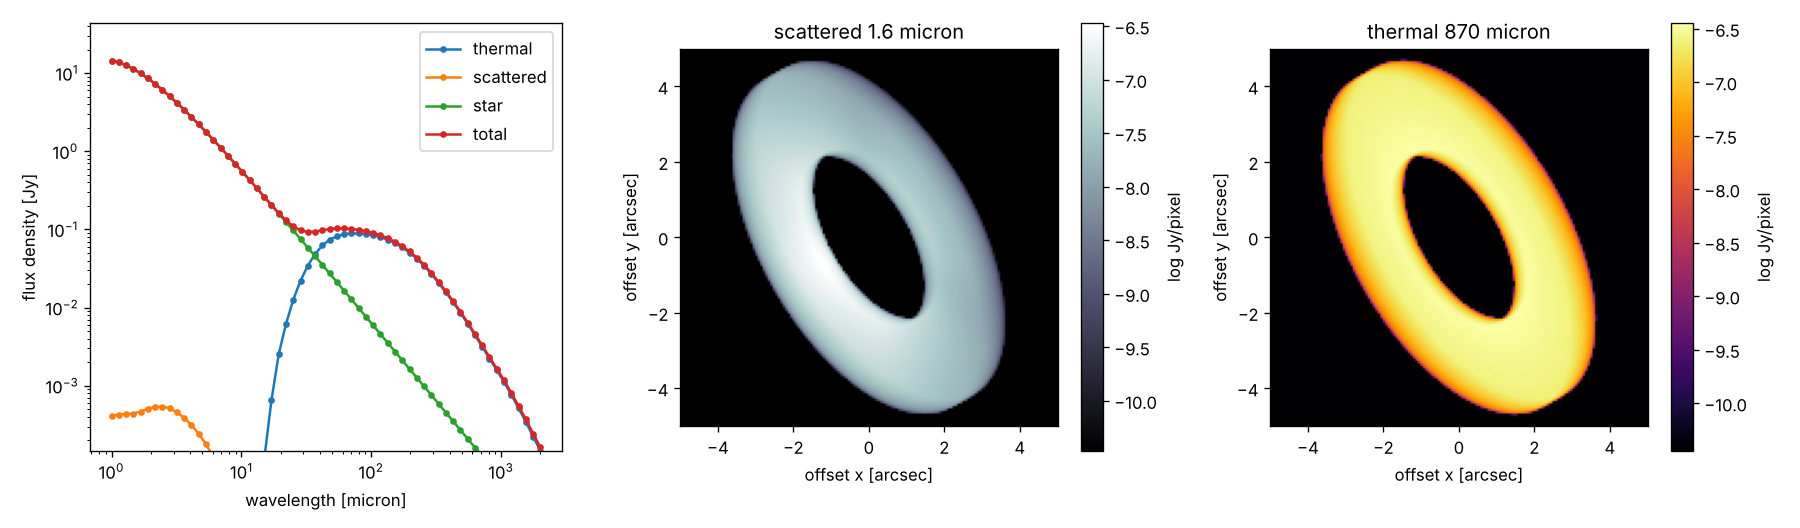
\includegraphics[width=\textwidth]{../images/quickstart.png}
\caption{Output of \code{examples/quickstart.py}: SED, scattered light at 1.6\um\ and thermal
emission at 870\um\ (logarithmic scale, Jy per pixel) of a ring between 50 and 100\,au around a
Sun-like star at 20\,pc.}
\label{fig:quickstart}
\end{figure}

\subsection{A more complete example}

\code{examples/two\_belts\_observed.py} (about two minutes) uses more of the code: a warm inner belt
(5--15\,au) and a cold eccentric outer belt (Gaussian, peak at 140\,au, $e=0.12$) around an A star
at 7.7\,pc; grains of silicate and water ice that turn into porous silicate above 110\,K; blow-out
for release at pericentre; a polarised-light image with a PSF and a coronagraph mask; thermal
images with a PSF. The dust and the three runs are

\begin{lstlisting}[style=py]
dust={"n_components": 2,
      "optical_data": ["kim2019/ice_astrosilicate_MG/Sil50cice50",   # silicate + ice
                       "kim2019/porous_astrosilicate/as50vac50"],    # residue
      "bulk_density": [1.95, 1.75], "abundance": [100, 0],
      "sublimation": True, "t_sublimation": [110, -1], "sublimation_residue": [2, 0],
      "a_min": 1, "a_max": 1000, "q": 3.5, "blowout_release": "pericentre"}

sed = system.copy().update(run={"mode": "sed"},
          wavelengths={"lambda_min": 1, "lambda_max": 2000, "n_lambda": 80}).run()
pol = system.copy().update(run={"mode": "image", "emission": "polarisation"},
          wavelengths={"lambda": [1.6]},
          image={"n_pixels": 201, "psf": "gaussian", "psf_fwhm": 0.2, "mask_radius": 2.5}).run()
th  = system.copy().update(run={"mode": "image", "emission": "thermal"},
          wavelengths={"lambda": [24, 870]},
          image={"n_pixels": 201, "psf": "gaussian", "psf_fwhm": [0.8, 0.4]}).run()
\end{lstlisting}

The blow-out threshold is $\beta\ge0.44$ in the outer belt ($(1-e)/2$) and 0.5 in the inner one;
icy grains smaller than about 6\um\ are removed. The ice of the remaining grains sublimates inside
21--27\,au, so the inner belt consists of porous silicate. Figure~\ref{fig:twobelts} shows the
results; the script also prints $f_\mathrm{d}=1.0\times10^{-4}$, the largest radial optical depth
($2.8\times10^{-3}$) and the flux densities.

\begin{figure}[!htb]
\centering
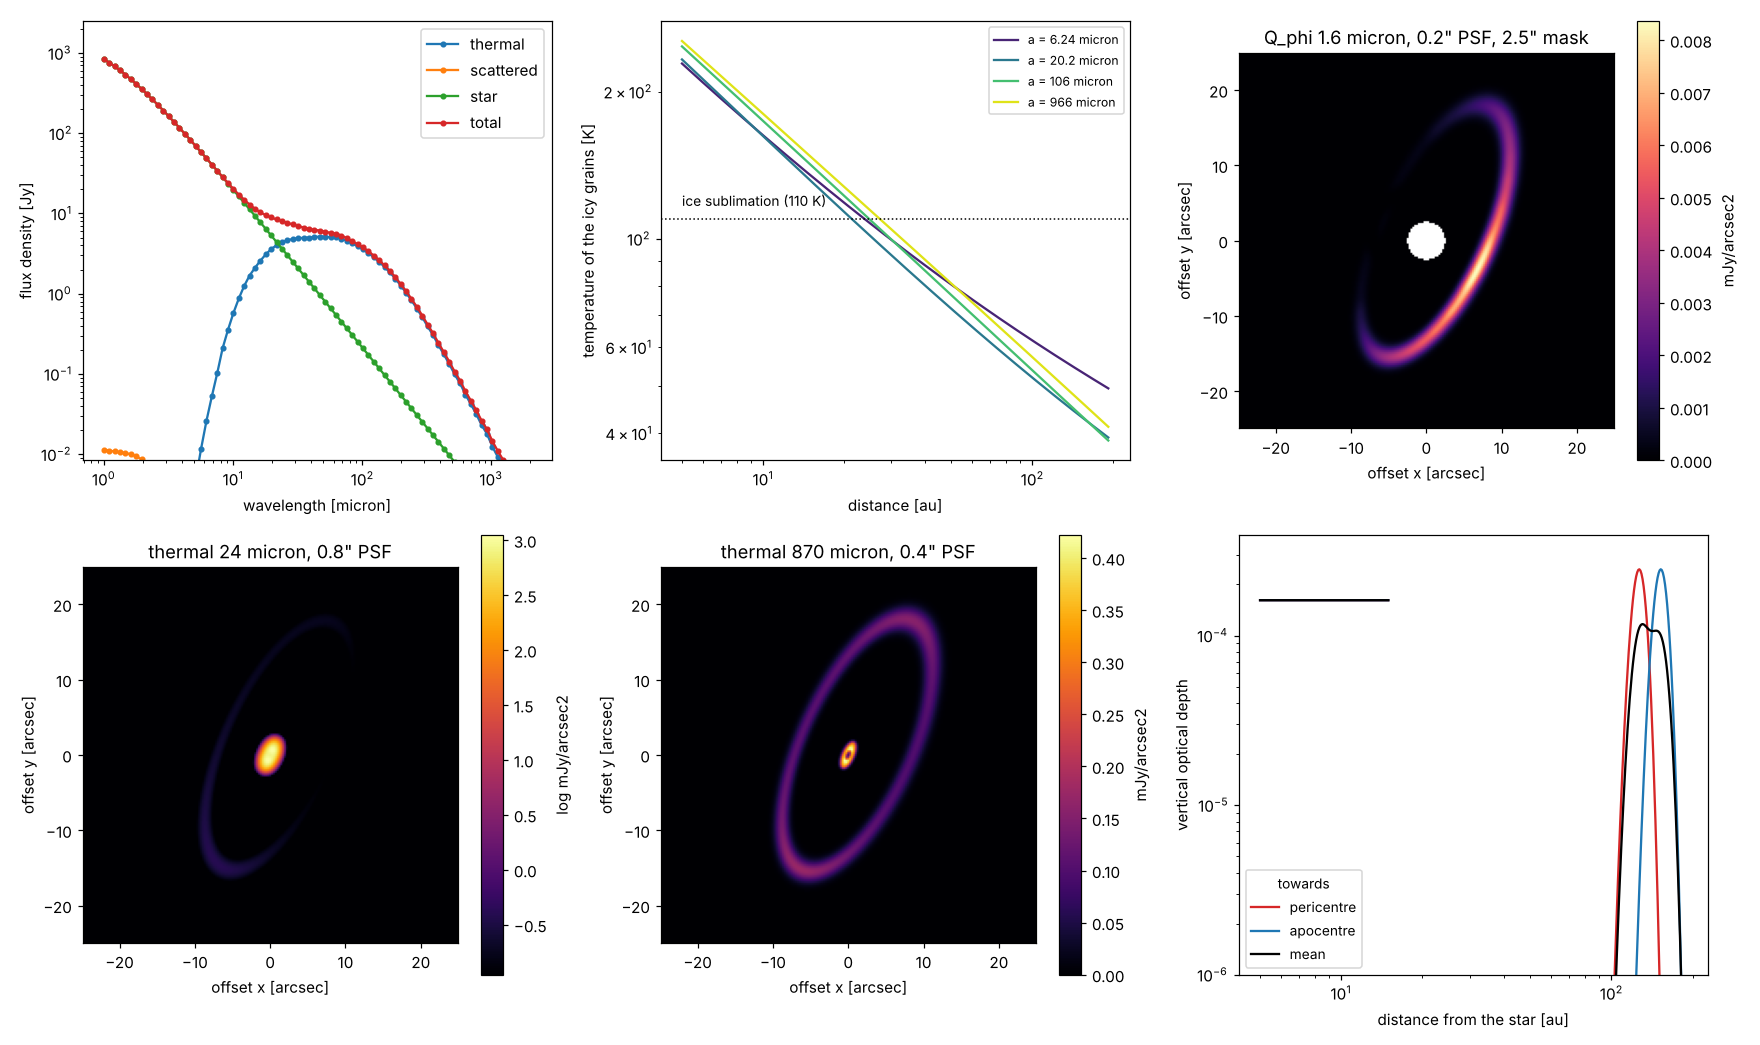
\includegraphics[width=\textwidth]{../images/two_belts_observed.png}
\caption{Output of \code{examples/two\_belts\_observed.py}. Top: SED; temperature of the icy grains
for four sizes (the smallest one left after blow-out, 20, 100 and 1000\um) with the sublimation
temperature; $Q_\phi$ at 1.6\um\ convolved with a 0.2$''$ PSF, with a coronagraph mask of
2.5$''$ radius. Bottom: thermal emission at 24\um\ (logarithmic scale) and 870\um\ convolved with
PSFs of 0.8$''$ and 0.4$''$; vertical optical depth towards pericentre and apocentre of the outer
belt and its azimuthal mean.}
\label{fig:twobelts}
\end{figure}
\FloatBarrier

\subsection{Running a model}

\begin{lstlisting}[style=py]
import dms

m = dms.Model.from_file("examples/debris_ring.nml")   # or dms.Model(star={...}, disk={...})
m.update(disk={"r_in": 60.0, "eccentricity": 0.1, "omega": 30.0},
         image={"n_pixels": 151, "psf": "gaussian", "psf_fwhm": 0.1})
res = m.run()                      # write_files=False, quiet=True by default

res.f_d, res.tau_mean              # fractional luminosity, mean optical depth
res.wavelength, res.sed["thermal"] # micron, Jy
img = res.image("Qphi", observed=True, unit="mJy/arcsec2")   # [n_wavelength, ny, nx]
m.write("model.nml")               # input file for the command-line program
\end{lstlisting}

Parameter names, units and groups are those of the input file. Lists are Python lists, e.g.\
\code{disk=\{"n\_belts": 2, "r\_in": [5, 80]\}}. An invalid input raises \code{dms.DMSError}, and
the Python session keeps running. A power-law size grid with fewer than 25 bins per decade gives a
\code{dms.SizeGridWarning} (Sect.~\ref{sec:perf}).

\subsection{The \code{Result} object}

\small
\begin{longtable}{@{}R{5.6cm}R{9.3cm}@{}}
\toprule
Attribute or method & Content \\
\midrule
\endhead
\code{wavelength} & observing wavelengths [\um] \\
\code{sed} & dict [Jy]: \code{thermal}, \code{scattered}, \code{Q}, \code{U}, \code{polarised},
  \code{star}, \code{total} \\
\code{image(name, observed, unit)} & cube [$n_\lambda$, $n_y$, $n_x$]; names \code{thermal},
  \code{scattered}, \code{Q}, \code{U}, \code{polarised}, \code{Qphi}, \code{Uphi},
  \code{poldeg}, \code{total} \\
\code{images} & names of the available images \\
\code{tau\_map}, \code{mass\_map\_kg} & line-of-sight optical depth, dust mass per pixel \\
\code{offsets("arcsec")} & pixel offsets along one axis \\
\code{f\_d}, \code{tau\_mean}, \code{tau\_peak} & global dust quantities \\
\code{blowout\_beta} & (smallest, largest) blow-out threshold used; (0, 0) if blow-out is off \\
\code{tau\_radial} & largest radial optical depth in the mid-plane ($>0.1$: optically thin
  assumption fails) \\
\code{tau\_profile} & \code{r\_au}, \code{mean}, \code{pericentre}, \code{apocentre} \\
\code{temperature} & \code{r\_au}, \code{T[n\_dist, n\_component, n\_size]} \\
\code{grains} & \code{a}, \code{edges}, \code{number}, \code{beta} \\
\code{luminosity\_lsun}, \code{pixel\_arcsec}, \code{pixel\_au} & stellar luminosity, pixel size \\
\code{phase\_curve(il, normalise)} & ($\theta$ [deg], $F_\mathrm{sca}$, $F_\mathrm{pol}$) of the
  whole disk in $1^\circ$ bins [Jy per bin] \\
\code{cube(name)} & \code{"reem"}, \code{"sca"}: [$n_\lambda$, $n_z$, $n_y$, $n_x$] in Jy;
  \code{"angle"}: scattering angle [$n_z$, $n_y$, $n_x$] (only with \code{save\_3d\_cubes}) \\
\bottomrule
\end{longtable}
\normalsize

\subsection{Fitting and parallel runs}

The Fortran state is global, so one model runs at a time in a Python process; OpenMP parallelises
inside the run. For many models at once (grids, MCMC with \code{emcee}), use separate processes
and set \code{OMP\_NUM\_THREADS=1} in each. The example below fits an observed SED on a small grid.
The guard \code{if \_\_name\_\_ == "\_\_main\_\_"} is required on macOS and Windows, where
\code{multiprocessing} starts new processes by importing the script.

\begin{lstlisting}[style=py]
import os
os.environ["OMP_NUM_THREADS"] = "1"          # before importing dms
from multiprocessing import Pool
import numpy as np
import dms

lam, f_obs, err = np.loadtxt("my_sed.txt", unpack=True)   # micron, Jy, Jy

def make_model(r_in=50.0, alpha=1.0):
    m = dms.Model.from_file("examples/debris_ring.nml")
    m.update(run={"mode": "sed", "load_optics": True, "save_optics": True,
                  "optics_cache_name": "fit"},
             wavelengths={"lambda": list(lam)},
             disk={"r_in": r_in, "alpha": alpha})
    return m

def chi2(params):
    sed = make_model(*params).run().sed["total"]
    return np.sum(((sed - f_obs) / err) ** 2)

if __name__ == "__main__":
    make_model().run()                       # computes and saves the optics once
    grid = [(r, a) for r in (40, 50, 60) for a in (0.0, 1.0, 2.0)]
    with Pool(8) as pool:
        values = pool.map(chi2, grid)
    print(grid[int(np.argmin(values))])
\end{lstlisting}

\subsection{Other modules}

\begin{itemize}
\item \code{dms.io}: read the output files of the command-line program (\code{read\_image},
      \code{read\_sed}, \code{read\_profile}, \code{read\_optical\_depth}).
\item \code{dms.plot}: quick-look plots of a \code{Result} (\code{image}, \code{sed},
      \code{temperature}).
\item \code{dms.namelist}: \code{read\_namelist}, \code{write\_namelist}.
\item \code{dms.stellar}, \code{dms.batch}, \code{dms.emc}: see the next section.
\end{itemize}

%----------------------------------------------------------------------------------------------------
\section{Grids of models, composite grains and stellar atmospheres}
\label{sec:tools}

\subsection{Batch runs: \code{dms.batch}}

\code{dms.batch} runs many models from a queue folder, several in parallel, and survives
interruptions.

\begin{lstlisting}[style=py]
import dms
from dms import batch

base = dms.Model.from_file("examples/debris_ring.nml")
jobs = batch.grid(base, {"disk.inclination": [0, 45, 70], "dust.q": [3.0, 3.5, 4.0]})
batch.write_queue(jobs, "queue")         # one input file per model
batch.run("queue", "runs", workers=8)    # returns when the queue is empty
table = batch.collect("runs")            # one row per model
\end{lstlisting}

From a terminal, which keeps running when a notebook is closed:

\begin{lstlisting}[style=sh]
python -m dms.batch run queue runs -j 8 --watch   # also picks up files added later
python -m dms.batch status queue
python -m dms.batch requeue queue                 # failed models back into the queue
touch queue/STOP                                  # ends a --watch run
\end{lstlisting}

A file being computed moves from \code{queue/} to \code{queue/running/} and then to
\code{queue/done/} or \code{queue/failed/}. Several runners, also on different machines sharing
the folder, can work on one queue, because a file is claimed by an atomic rename. Each model writes
into \code{runs/<name>/}: the \dms\ output, \code{input.nml}, \code{dms.log}, \code{meta.json} and
\code{result.json} (wavelengths, SED, degree of polarisation against scattering angle, and the
disk-integrated $Q_\phi/I$ if images were made). With \code{optics\_cache\_name = 'auto'}, models
that differ only in geometry, star or $q$ share one optical-property cache, and the runner never
starts two models that would compute the same cache at the same time.

\subsection{Composite grains: \code{dms.emc}}
\label{sec:emcuse}

\code{dms.emc.mix} runs \code{emc} (Ossenkopf 1991) without its interactive menus and writes a
\dms\ optical-data file. The executable is given with \code{emc=...} or the environment variable
\code{DMS\_EMC}.

\begin{lstlisting}[style=py]
from dms import emc
C = emc.Component
emc.mix("bruggeman",
        [C("astrosilicate_draine03_862", 0.5, "sphere"),
         C("kim2019/pure_ices/composite_aice.txt", 0.5, "needle")],
        "data/optical_constants/mixtures/as_aice_bg.txt")
\end{lstlisting}

Theories are \code{'maxwell-garnett'}, \code{'bruggeman'}, \code{'uni-mg'} and \code{'uni-bg'};
shapes are \code{'host'}, \code{'sphere'}, \code{'needle'}, \code{'platelet'}, \code{'coated'}
(with \code{mantle=}), \code{'coating'} and \code{'shape'} (with a depolarisation factor
\code{L=}). The name \code{'vacuum'} selects the built-in vacuum of \code{emc}, for porous grains.
\code{grid\_from=i} takes the wavelength grid of the result from component $i$. For a grain made
only of core and mantle, \code{'uni-mg'} and \code{'uni-bg'} give the same result, since both
reduce to the coated-sphere formula.

\subsection{Model-atmosphere grids: \code{dms.stellar}}
\label{sec:grids}

A grid directory contains \code{grid\_index.txt} (lines with $T_\mathrm{eff}$, $\log g$ and a file
name) and one file per model with wavelength [\um] and surface flux $F_\lambda$
[W\,m$^{-2}$\,m$^{-1}$]. Grids are built with (internet access required):

\begin{lstlisting}[style=sh]
python -m dms.stellar ck04    data/stellar_models/ck04_p00   --teff 4000 10000 --logg 3.5 5.0
python -m dms.stellar phoenix data/stellar_models/phoenix_z0 --teff 3000 7000  --logg 4.0 5.0
python -m dms.stellar blackbody data/stellar_models/bb --teff 3000 10000
\end{lstlisting}
and used with
\code{\&star spectrum = 'grid', grid\_dir = 'data/stellar\_models/ck04\_p00', teff = 5770.,
logg = 4.44 /}. Please cite Castelli \& Kurucz (2004) or Husser et al.\ (2013) for the grid you
use. The download routines have not yet been tested against the archive servers; reading and
interpolating a grid was tested with black-body grids.

%----------------------------------------------------------------------------------------------------
\section{Performance and accuracy}
\label{sec:perf}

\begin{itemize}
\item \textbf{Optical properties dominate} a single run. Save them once (\code{save\_optics}) and
      reuse them (\code{load\_optics}) while the grains, wavelengths and optical data stay the
      same; the cache is ignored automatically when any of these change. DHS is 10--20 times
      slower than compact spheres.
\item \textbf{SED first.} \code{mode = 'sed'} is much faster than images and gives the same SED.
\item \textbf{Image resolution.} The time scales with the number of pixels and the refinement.
      Start with 101 pixels and $N_\mathrm{max}=3$. Increase $N_\mathrm{max}$ for thin edge-on disks
      and narrow belts, and check that the result changes by less than your tolerance.
\item \textbf{Temperature criterion.} \code{max\_delta\_t = 2} is adequate for most cases. For hot
      inner dust a smaller value refines more near the star.
\item \textbf{Size bins.} Each size bin is represented by one grain size. Mie polarisation of
      large grains oscillates with grain size, and a coarse size grid leaves radial stripes in
      $Q_\phi$ images. The thermal emission at (sub)millimetre wavelengths comes from grains with
      $2\pi a\sim\lambda$, whose absorption efficiency changes quickly with $\lambda/a$; on a
      coarse grid the SED then ripples with the period of the size grid. For the quick-start model
      of Sect.~\ref{sec:python} (1--1000\um, $q=3.5$, astronomical silicate) the largest deviation between 100 and 2000\um\ from a
      400-bin calculation is 29\,\% with 30 bins (10 per decade; 16\,\% at 870\um), 12\,\% with
      60 bins and 4\,\% with 100 bins. Use at least 30 bins per decade for Mie polarisation images
      and for (sub)millimetre fluxes; the default of 100 bins gives 33 per decade for 1--1000\um.
      Below 25 bins per decade \dms\ prints a note, and the Python interface issues a
      \code{dms.SizeGridWarning}.
\item \textbf{Angles.} Use more than 181 angles when large grains at short wavelengths make the
      forward peak narrow and the forward-scattering side of the disk matters.
\item \textbf{Threads.} \code{OMP\_NUM\_THREADS} sets the number of threads of one run; for batches,
      prefer one thread per model and many models in parallel.
\end{itemize}

%----------------------------------------------------------------------------------------------------
\section{Troubleshooting}
\label{sec:trouble}

\small
\begin{longtable}{@{}R{6.1cm}R{8.8cm}@{}}
\toprule
Message or problem & Cause and remedy \\
\midrule
\endhead
\code{input file not found} & Wrong path; paths are relative to the working directory. \\
\code{error in namelist group \&disk} & Misspelt parameter name or a missing quote; the compiler
  message after the colon names the problem. \\
\code{observing wavelengths must lie within the wavelength range of the optical data} & Choose
  wavelengths inside the range shared by all optical-data files (printed in the message). \\
\code{no grains left: all grain sizes are blown out} & Every size bin has $\beta\ge0.5$. Increase
  \code{a\_min} or \code{a\_max}, or switch \code{blowout} off. \\
\code{no grains left after sublimation / blow-out} & Check \code{t\_sublimation}, the residues,
  \code{a\_min} and the belt radii. \\
\code{no dust inside the model space} & The belt radii, opening angle or field do not contain dust;
  check the \code{\&disk} parameters. \\
\code{blow-out requires a positive stellar mass} & Set \code{\&star mass}. \\
\code{give either blowout\_beta or blowout\_release} & Use one of the two inputs. \\
\code{Mie calculation failed} & Size parameter beyond the limit of the Mie routine (very large grains
  at very short wavelengths, or very small grains at very long ones). Reduce the range. \\
\code{T\_eff ... is outside the model grid} & Extend the grid or change $T_\mathrm{eff}$, $\log g$. \\
Images look blocky near the star & Increase \code{n\_split\_max} or decrease \code{max\_delta\_t}. \\
\code{ImportError: compiled DMS extension is missing} & Run \code{make python}; with Python 3.12 or
  later install \code{meson} and \code{ninja} first. \\
\code{make python} fails with OpenMP symbols & Build everything without OpenMP:
  \code{make serial}, then \code{make python OMP=""}. Otherwise make sure that \code{gfortran} and
  the compiler used by Python belong to the same toolchain. \\
Results differ between machines & Different compilers or \code{-march=native}; differences should be
  at the level of rounding. \\
\bottomrule
\end{longtable}
\normalsize

%----------------------------------------------------------------------------------------------------
\section{Extending \dms}
\label{sec:extend}

\subsection{Your own density distribution}

Edit \code{src/user\_density.f90} and recompile (\code{make}; for Python also \code{make python}).
The function receives the semi-major axis $\mathcal{A}$ [m], the disk-frame coordinates $X,Y,Z$
[m], the belt number and the ten parameters \code{user\_par}, and returns a non-negative relative
density. \dms\ applies the belt limits, the factor $\mathcal{A}/s$ of eccentric belts and the
vertical profile itself. The default is a power law times a Gaussian clump:

\begin{lstlisting}[language=Fortran, style=base]
psi   = atan2(X, Y)                                     ! azimuth in the disk plane
dpsi  = modulo(psi - par(3) * deg2rad + pi, 2.0_r2 * pi) - pi
width = max(par(4), 1.0e-3_r2) * deg2rad
rho   = (a / au)**(-par(1)) * (1.0_r2 + par(2) * exp(-0.5_r2 * (dpsi / width)**2))
\end{lstlisting}

If the distribution is symmetric under $Y\to-Y$, set \code{user\_density\_symmetric = .true.} to
halve the computing time of images.

\subsection{Adding an input parameter}

\begin{enumerate}
\item Declare it in \code{parameters.f90}; set its default in \code{set\_defaults} and check it in
      \code{finalize\_input} (\code{input\_setup.f90}).
\item Add it to the namelist in \code{read\_input\_file.f90} and, if relevant, to the interactive
      questions.
\item Release new allocatable arrays in \code{dms\_reset.f90}.
\item Document it in \code{docs/input\_reference.md} and in this manual.
\end{enumerate}
Errors are reported with \code{call dms\_fail("message")} followed by \code{return}; \code{stop}
must not be used, so that the Python interface survives invalid input. The routines called inside
the OpenMP loops must only read global variables. Every new feature gets a test in \code{tests/}.
Before a pull request, \code{make debug} must compile without warnings and \code{make test} must
pass; GitHub Actions repeats both.

%----------------------------------------------------------------------------------------------------
\section{Citing, licence and acknowledgements}
\label{sec:cite}

If you use \dms, please cite Kim et al.\ (2018) and, if one is given for the release you use, the
DOI of that release (see the repository page). If you use the optical data in
\code{data/}\allowbreak\code{optical\_constants/}, please also cite the references given there (for the water-ice
data: Kim et al.\ 2019 and the original laboratory measurements). The file \code{CITATION.cff}
lets GitHub show a citation for the repository.

\paragraph{Third-party code.} The Mie routine \code{miex} in \code{src/mie\_routines.f90} was
written by Wolf \& Voshchinnikov (2004) and adapted for \dms\ 2.0 (Sect.~\ref{sec:optics}); its
authors set the terms under which it may be redistributed. The coated-sphere and DHS routines in the
same file implement the algorithms of Yang (2003) and Min et al.\ (2005). The
code \code{emc} (Ossenkopf 1991) is not distributed with \dms; \code{dms.emc} calls a copy
installed by the user.

\paragraph{Acknowledgements.} I thank Steve Ertel, Robert Brunngr\"aber, Florian Kirchschlager,
Sebastian Wolf and Thomas Stuber for their help with the original version of the code.

%----------------------------------------------------------------------------------------------------
\section*{About the cover}
\addcontentsline{toc}{section}{About the cover}
\markboth{About the cover}{About the cover}
\label{sec:cover}

All eight images on the cover were computed with \dms\ 2.0 at $401\times401$ pixels. The input of
every model is in \code{docs/}\allowbreak\code{manual/}\allowbreak\code{cover/}\allowbreak\code{cover\_models.py},
and \code{cover\_images.py} in the same folder turns them into the eight images in
\code{cover/}\allowbreak\code{images/}; \code{README.md} there explains how to reproduce them. The
cover page itself (title, captions and layout) is set at the start of \code{dms\_manual.tex}. All models use astronomical silicate (Draine 2003) with grain radii from 1 to
1000\um, $q=3.5$ and Mie theory. Only the display was added after \dms: every image is divided by
a value close to its maximum (the 99.9th percentile of its pixels) and shown with a logarithmic or
power-law stretch.

\begin{center}
\small
\begin{tabularx}{\textwidth}{@{}R{3.6cm}X@{}}
\toprule
Panel & Model \\
\midrule
Scattered light and $Q_\phi$, 1.6\um &
  Gaussian ring, $\mu=78$\,au, $\sigma=3$\,au, Gaussian vertical profile with $h/r=0.02$,
  $i=76^\circ$; star with $T_\mathrm{eff}=9500$\,K at 72\,pc. The near side (upper left) is
  brighter because the grains scatter mainly forwards. \\
Edge-on disk, 1.6\um &
  Broken power law (\code{'broken'}), rising as $\mathcal{A}^{5}$ inside 90\,au and falling as
  $\mathcal{A}^{-3}$ outside, $h/r=0.05$, $i=87^\circ$. \\
Two belts, 24/70/870\um &
  Inner belt 8--20\,au (3\,\% of the dust mass) and outer Gaussian belt with $\mu=140$\,au,
  $\sigma=10$\,au and $e=0.12$, $i=55^\circ$. Red, green and blue show 870, 70 and 24\um; one
  logarithmic stretch of the summed intensity keeps the colour (Lupton et al.\ 2004). \\
Pericentre and apocentre glow, 24 and 870\um &
  Ring with $\mathcal{A}=136$--140\,au, $e=0.3$, $i=20^\circ$, at 7.7\,pc; both images
  convolved by \dms\ with a Gaussian PSF of 1.5$''$ FWHM (\code{psf = 'gaussian'}), wider than
  the ring. The apocentre-to-pericentre ratio of the peak brightness is 0.22 at 24\um\ and 1.24 at
  870\um\ (Sect.~\ref{sec:geometry}). Apocentre glow was first detected conclusively in the
  ALMA map of Fomalhaut (MacGregor et al.\ 2017). \\
Belt with a gap, 870\um &
  User-defined density (\code{user\_density\_cover.f90}, \code{user\_par(10) = 1}):
  $n\propto 1-0.5\exp[-(\mathcal{A}-80\,\mathrm{au})^2/2(10\,\mathrm{au})^2]$ between 40 and
  140\,au, similar in size to the gap in the belt of HD~107146 (Marino et al.\ 2018). \\
Ring with a clump, 870\um &
  The example shipped in \code{src/user\_density.f90} (Sect.~\ref{sec:extend}):
  $n\propto\mathcal{A}^{-1}[1+2\exp(-\Delta\psi^2/2\cdot25^{\circ\,2})]$, ring 50--90\,au. Planets
  that migrate outwards can trap planetesimals in mean-motion resonances and produce such clumps
  (Wyatt 2003). \\
\bottomrule
\end{tabularx}
\end{center}

%----------------------------------------------------------------------------------------------------
\section*{References}
\addcontentsline{toc}{section}{References}
\markboth{References}{References}
\small
\begin{list}{}{\leftmargin=1.2em \itemindent=-1.2em \itemsep=1pt}
\item Augereau J.-C., Lagrange A.-M., Mouillet D., Papaloizou J.~C.~B., Grorod P.~A., 1999, A\&A, 348, 557
\item Bohren C.~F., Huffman D.~R., 1983, Absorption and Scattering of Light by Small Particles. Wiley, New York
\item Burns J.~A., Lamy P.~L., Soter S., 1979, Icarus, 40, 1
\item Castelli F., Kurucz R.~L., 2004, arXiv:astro-ph/0405087
\item Dorschner J., Begemann B., Henning Th., J\"ager C., Mutschke H., 1995, A\&A, 300, 503
\item Draine B.~T., 2003, ApJ, 598, 1026
\item Dullemond C.~P., Juhasz A., Pohl A., et al., 2012, RADMC-3D, Astrophysics Source Code Library, ascl:1202.015
\item Engler N., et al., 2017, A\&A, 607, A90
\item Ertel S., Wolf S., Metchev S., et al., 2011, A\&A, 533, A132
\item Ertel S., Wolf S., Marshall J.~P., et al., 2012, A\&A, 541, A148
\item Henning Th., Stognienko R., 1996, A\&A, 311, 291
\item Henyey L.~G., Greenstein J.~L., 1941, ApJ, 93, 70
\item Husser T.-O., et al., 2013, A\&A, 553, A6
\item Kim M., Wolf S., L\"ohne T., Kirchschlager F., Krivov A.~V., 2018, A\&A, 618, A38
\item Kim M., Wolf S., Potapov A., Mutschke H., J\"ager C., 2019, A\&A, 629, A141
\item Lupton R., Blanton M.~R., Fekete G., Hogg D.~W., O'Mullane W., Szalay A., Wherry N., 2004, PASP, 116, 133
\item MacGregor M.~A., Matr\`a L., Kalas P., et al., 2017, ApJ, 842, 8
\item Marino S., Carpenter J., Wyatt M.~C., et al., 2018, MNRAS, 479, 5423
\item Mastrapa R.~M., Bernstein M.~P., Sandford S.~A., Roush T.~L., Cruikshank D.~P., Dalle Ore C.~M., 2008, Icarus, 197, 307
\item Mastrapa R.~M., Sandford S.~A., Roush T.~L., Cruikshank D.~P., Dalle Ore C.~M., 2009, ApJ, 701, 1347
\item Min M., Hovenier J.~W., de Koter A., 2005, A\&A, 432, 909
\item Min M., Rab C., Woitke P., Dominik C., M\'enard F., 2016, A\&A, 585, A13
\item Ossenkopf V., 1991, A\&A, 251, 210
\item Pan M., Nesvold E.~R., Kuchner M.~J., 2016, ApJ, 832, 81
\item Pe\~na O., Pal U., 2009, Comput. Phys. Commun., 180, 2348
\item Pinte C., M\'enard F., Duch\^ene G., Bastien P., 2006, A\&A, 459, 797
\item Robitaille T.~P., 2011, A\&A, 536, A79
\item Wolf S., Voshchinnikov N.~V., 2004, Comput. Phys. Commun., 162, 113
\item Wyatt M.~C., 2003, ApJ, 598, 1321
\item Yang W., 2003, Appl. Opt., 42, 1710
\item Zubko V.~G., Mennella V., Colangeli L., Bussoletti E., 1996, MNRAS, 282, 1321
\end{list}

\end{document}
